\documentclass[a4paper,10pt]{scrreprt}

% Seitenr�nder
\usepackage[top=2.0cm,bottom=2.0cm,left=1.5cm,right=2.5cm]{geometry}

% Encoding + Sprache
\usepackage[ngerman]{babel}
\usepackage[ansinew]{inputenc}
\usepackage[T1]{fontenc}

% Captions
\usepackage{caption}

% Farben/Grafik
\usepackage[table]{xcolor}
\usepackage{graphicx}
\definecolor{violett}{RGB}{154,50,205}
\definecolor{darkgreen}{RGB}{0,136,0}
\definecolor{htwgreen}{RGB}{134,189,36}

% Mathe
\usepackage{amssymb}
\usepackage{amsmath}
\usepackage{amstext}
\usepackage{amsfonts}

% Tabellen
\usepackage{float}
\usepackage{booktabs}
\usepackage{tabularx}
\usepackage{array} % f�r Tabellenspalten, falls n�tig

\newcommand{\tabitem}{~~\llap{\textbullet}~~}

% codeboxes
\usepackage{listings}
\lstset{basicstyle=\small\ttfamily,breaklines=true,columns=fullflexible,keepspaces=true}

% tcolorbox
\usepackage{tcolorbox}
\tcbuselibrary{breakable,skins}

% Hyperref (sp�ter laden, aber vor scrlayer-scrpage)
\usepackage{hyperref}
\hypersetup{
  colorlinks = true,
  urlcolor   = red,
  linkcolor  = red,
  citecolor  = red
}

% Einmal in der Praeambel des Hauptdokuments nach hyperref laden.
% true: Theorie, Aufgaben und Loesungen gemeinsam; false: getrennte Ausgaben.
\newif\ifintegriereaufgaben
\integriereaufgabenfalse

% Fuehrt den gesamten Inhalt nur bei vorhandenem Label aus.
% Wie normale Querverweise benoetigt die Erkennung mehrere LaTeX-Laeufe.
\newcommand{\wennreferenzvorhanden}[2]{%
  \ifcsname r@#1\endcsname
    #2%
  \fi
}

% Verlinkte Nummer bei vorhandenem Ziel, andernfalls keinerlei Ausgabe.
\newcommand{\abschnittsverweis}[1]{%
  \wennreferenzvorhanden{#1}{\ref{#1}}%
}

% Gleichbedeutender Name fuer bestehende Theoriehinweise.
\newcommand{\skriptverweis}[1]{\abschnittsverweis{#1}}

% Ohne Ziel wird auch kein leerer Randnotiz-Kasten angelegt.
\newcommand{\randverweis}[1]{%
  \wennreferenzvorhanden{#1}{\marginpar{\small\abschnittsverweis{#1}}}%
}

\integriereaufgabenfalse

% KOMA-Script header/footer
\usepackage{scrlayer-scrpage}
\clearpairofpagestyles
\cfoot*{\footnotesize
Prof. Dr. Lucy Weggler -- Lizenz:
\href{https://creativecommons.org/licenses/by-nc-sa/4.0/}{CC-BY-NC-SA 4.0}
}

\ofoot*{\pagemark}
\titlehead{\thispagestyle{plain.scrheadings}}

% Gemeinsame Kopfzeile: eine Hauptueberschrift, links, klein und aufrecht.
% Die Fusszeilen werden weiterhin im jeweiligen Hauptdokument festgelegt.
\makeatletter
\@ifpackageloaded{scrlayer-scrpage}{%
  % Im gegliederten Gesamtskript ist das Kapitel die Hauptueberschrift.
  \automark{chapter}
  \setkomafont{pagehead}{\normalfont\footnotesize}
  \ihead{}\chead{}\ohead{}
  \lehead{\headmark}
  \lohead{\headmark}
}{%
  % In den article-Dokumenten ist section die oberste Gliederungsebene.
  \fancyhead{}
  \fancyhead[L]{\normalfont\footnotesize\nouppercase{\leftmark}}
  \renewcommand{\sectionmark}[1]{\markboth{\thesection\quad #1}{}}
  \renewcommand{\subsectionmark}[1]{}
  \setlength{\headheight}{14pt}
}
\makeatother

% --- tcolorbox-Definitionen ---------------------
% Definition
% #1: Title
% #2: Bemerkung
\newcounter{def}
\newtcolorbox{defbox}[3][]{
  enhanced,
  overlay unbroken and first={
\node[fill=white,rounded corners, draw=white, text=gray, line width=3pt, inner sep=4pt, anchor=east, xshift=-10pt] at (frame.north east){#2};
\node[anchor=north east, text=gray, fill=white, text width=3.5em, align=left, minimum height=4ex] at ([xshift=4.5\marginparsep]frame.north east) {\small Def. \stepcounter{def}\thedef \newline \textcolor{black}{#3} };
},
  colframe=gray,
  %colback=mytestcolor,
  colback=white,
  coltitle=red!70!gray,
  boxrule=1pt,
  arc=1mm,
  breakable,
  top=5pt,
  before=\vskip18pt}

% Satz
% #1: Title
% #2: Bemerkung
\newcounter{satz}
   \newtcolorbox{theorembox}[3][]{
  enhanced,
  overlay unbroken and first={
\node[fill=white,rounded corners, draw=white, text=gray, line width=3pt, inner sep=4pt, anchor=east, xshift=-10pt] at (frame.north east){#2};
\node[anchor=north east, text=gray, fill=white, text width=3.5em, align=right, minimum height=4ex] at ([xshift=4.5\marginparsep]frame.north east) {\small Regel \stepcounter{satz}\thesatz \newline \textcolor{black}{#3} };
},
  colframe=gray,
  %colback=mytestcolor,
  colback=white,
  coltitle=red!70!gray,
  boxrule=1pt,
  arc=1mm,
  breakable,
  top=5pt,
  before=\vskip18pt
}

% Beispiel
% #1: Title
% #2: Bemerkung
\newcounter{exa}
\newtcolorbox{exabox}[3][]{
  enhanced,
  overlay unbroken and first={
	  \node[fill=white, rounded corners, draw=white, text=blue, line width=3pt, inner sep=4pt, anchor=east, xshift=-10pt] at (frame.north east) {#2};
	  \node[anchor=north east, text=blue, fill=white, text width=3.5em, align=right, minimum height=4ex] at ([xshift=4.5\marginparsep]frame.north east)  {\small  Bsp \stepcounter{exa}\theexa \newline \textcolor{black}{ #3} };
},
  colframe=blue,
  colback=white,
  coltitle=red!70!blue,
  boxrule=1pt,
  arc=1mm,
  breakable,
  top=5pt,
  before=\vskip18pt
}

% Nummerierung
\makeatletter
\@addtoreset{chapter}{part}
\makeatother

\begin{document}
\title{Mathematik f�r Ingenieure\\ \vspace{0.5cm} {Ein Einstieg in Multivariate Analysis}}
\author{Prof. Dr. Lucy Weggler (HTW Berlin)}
\date{\today}
\maketitle
\setcounter{page}{2}

\tableofcontents
\cleardoublepage

\setcounter{def}{0} \setcounter{satz}{0} \setcounter{exa}{0}
\chapter{Funktionen mehrerer Ver�nderlicher}\label{MULTI-funktionen-mehrerer-veraenderlicher}

\begin{table}[H]
  \centering
  \begin{tabularx}{\textwidth}{@{}>{\raggedright\arraybackslash}X r@{}}
    \toprule
    \multicolumn{2}{c}{\textbf{�bersicht �ber Lernziele und Voraussetzungen}}\\
    \midrule
    \textbf{Lernziele} & \\[.5\normalbaselineskip]
    \tabitem Funktionen mehrerer Ver�nderlicher geometrisch interpretieren (Graph, H�henlinien) & \\
    \tabitem partielle Ableitungen berechnen & \\
    \tabitem den Gradienten einer Funktion bestimmen und geometrisch deuten & \\
    \tabitem die Tangentialebene als lineare N�herung einer Funktion aufstellen & \\
    \tabitem das totale Differential formulieren und anwenden & \\[.5\normalbaselineskip]
    \midrule
    \textbf{Voraussetzungen} & \\[.5\normalbaselineskip]
    \tabitem Ableitungen von Funktionen einer Ver�nderlichen &  \\
    \tabitem lineare N�herungen (Tangente) & \\
    \tabitem Vektoren und Skalarprodukte & \\[.5\normalbaselineskip]
    \bottomrule
  \end{tabularx}
\end{table}

\section*{Leitidee}

Funktionen mehrerer Ver�nderlicher beschreiben Zusammenh�nge, bei denen ein Ergebnis gleichzeitig von mehreren Einflussgr��en abh�ngt. In technischen Anwendungen ist das der Normalfall: Eine Gr��e h�ngt etwa von Ort, Zeit, Temperatur, Druck oder mehreren geometrischen Parametern ab.

Die entscheidende neue Frage lautet:
\begin{center}
\textbf{Wie �ndert sich eine Funktion, wenn man sich von einem Punkt aus in verschiedene Richtungen bewegt?}
\end{center}

Bei Funktionen einer Ver�nderlichen gibt es nur eine unabh�ngige Richtung. Bei Funktionen mehrerer Ver�nderlicher gibt es dagegen unendlich viele m�gliche Bewegungsrichtungen. Deshalb muss man genauer unterscheiden:
\begin{itemize}
\item Wie stark �ndert sich die Funktion entlang der Koordinatenachsen?
\item In welche Richtung w�chst sie am st�rksten?
\item Wie kann man ihr Verhalten in einer Umgebung eines Punktes durch ein lineares Modell approximieren?
\end{itemize}

Die zentralen Werkzeuge dazu sind die partiellen Ableitungen, der Gradient, die Jacobi-Matrix und die Tangentialebene. Sie erlauben es, das lokale Verhalten einer Funktion systematisch zu beschreiben und bilden die Grundlage f�r Fehlerabsch�tzung, Optimierung, Koordinatentransformationen und mehrdimensionale Integration.

\section{Vektorfelder}

Die �bliche Vorstellung, die man von einer (reellwertigen) Funktion zwei reeller Ver�nderlicher hat, ist die eines Gebirges: die Funktion ordnet jedem Punkt in der \((x,y) \)-Ebene seine H�he zu. Die H�he ist dann die zu \(x\) und \(y\) geh�rige \(z\)-Koordinate. Das Tripel \( (x,y,z)\) lebt also in drei Dimensionen und ist ein Punkt auf einer im Allgemeinen beliebig gekr�mmten Fl�che im Raum:
\begin{figure}[h]
\centering
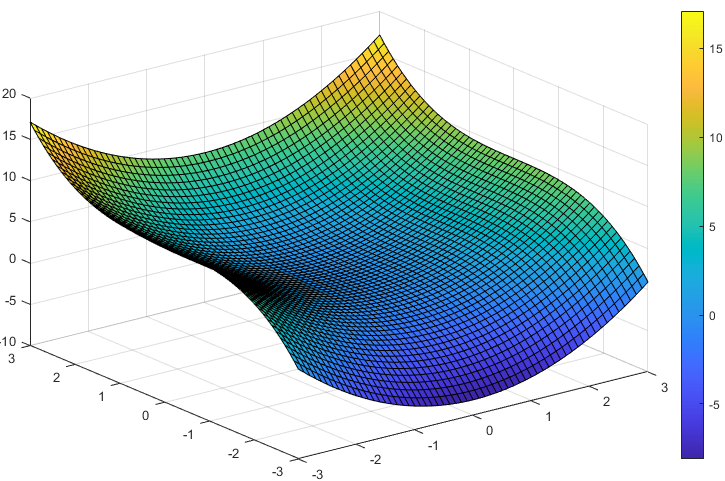
\includegraphics[width=0.6\textwidth]{../Multivariate_Analysis/Bilder/funktion_polynom_oberflaeche.png}
\caption{Visualisierung \(f(x,y)=x^2+0.3\,y^3\) als Oberfl�che in \(\mathbb R^3\).}
\end{figure}

\begin{center}
\begin{tabular}{p{0.45\textwidth}|p{0.45\textwidth}}

\textbf{Matlab} &
\textbf{Python} \\

\begin{lstlisting}[language=Matlab]
x = -3:0.1:3;
y = -3:0.1:3;
[xx,yy] = meshgrid(x,y);
z = xx.^2+0.3*yy.^3;
surf(x,y,z)
colorbar
\end{lstlisting}

&
\begin{lstlisting}[language=Python]
import numpy as np
import matplotlib.pyplot as plt

x = np.arange(-3,3.1,0.1)
y = np.arange(-3,3.1,0.1)
xx,yy = np.meshgrid(x,y)
z = xx**2 + 0.3*yy**3

fig = plt.figure()
ax = fig.add_subplot(projection='3d')
surf = ax.plot_surface(xx,yy,z)
fig.colorbar(surf)
plt.show()
\end{lstlisting}

\end{tabular}
\end{center}

M�chte man ein Gebirge auf einem Blatt Papier zeichnen, dann �bersetzt man oft die \(z\)-Koordinate in eine Farbe (Matlab \verb-imagesc-) oder man zeichnet \textbf{ H�henlinien } (Isolinien, �quipotentialinien):

\begin{figure}[h]
\centering
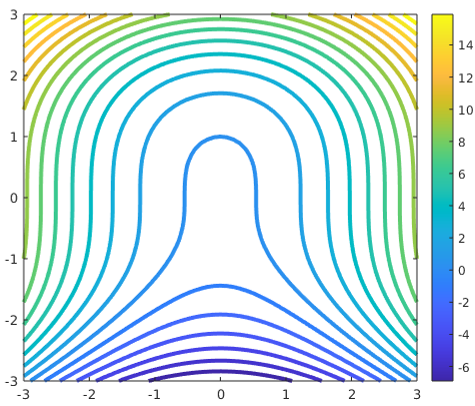
\includegraphics[width=0.6\textwidth]{../Multivariate_Analysis/Bilder/funktion_polynom_hoehenlinien.png}
	\caption{Visualisierung \(f(x,y)=x^2+0.3\,y^3\) als H�henlinienprofil in \(\mathbb R^2\).}
\end{figure}

\vspace{0.5cm}

\begin{center}
\begin{tabular}{p{0.45\textwidth}|p{0.45\textwidth}}

\textbf{Matlab} &
\textbf{Python} \\

\begin{lstlisting}[language=Matlab]
x = -3:0.1:3;
y = -3:0.1:3;
[xx,yy] = meshgrid(x,y);
z = xx.^2 + 0.3*yy.^3;
contour(x,y,z,20,'LineWidth',2)
colorbar
\end{lstlisting}

&
\begin{lstlisting}[language=Python]
import numpy as np
import matplotlib.pyplot as plt

x = np.arange(-3, 3.1, 0.1)
y = np.arange(-3, 3.1, 0.1)
xx, yy = np.meshgrid(x, y)

z = xx**2 + 0.3*yy**3

plt.contour(x, y, z, 20, linewidths=2)
plt.colorbar()
plt.show()
\end{lstlisting}

\end{tabular}
\end{center}
\vspace{0.5cm}

Eine Funktion $f$ von $n$ Ver�nderlichen ordnet einem Punkt $\vec x = (x_1,x_2,\cdots,x_n)^\intercal$ mit \(n\) Koordinaten genau einen Wert zu. Der Definitionsbereich (\emph{domain}) von \(f\) ist also eine Teilmenge des \(\mathbb R^n\) und der Zielbereich sind die reellen Zahlen:
\[ f: D_f\subset \mathbb R^n \to \mathbb R, \vec x \mapsto f(\vec x)\,.\]
Die Menge der tats�chlich vorkommenden Werte $f(\vec x)$ hei�t, wie im Falle \(n=1\), das Bild oder der Bildbereich (\emph{image} oder \emph{range}) der Funktion $f$, kurz $f(D_f)$. Wie f�r Funktionen einer Ver�nderlicher ist das Bild der Funktion eine Untermenge des Zielbereichs (\emph{codomain}).
\begin{exabox}{Definitionsbereich und Bild einer zweidimensionalen Funktion }{}
	\begin{minipage}{0.4\textwidth}
		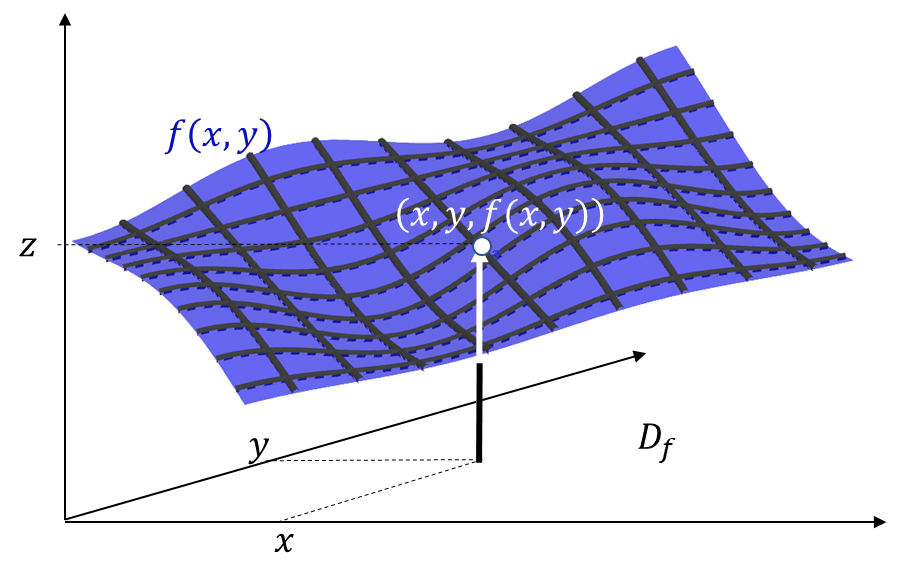
\includegraphics[width=\textwidth]{../Multivariate_Analysis/Bilder/funktion_definitionsbereich_und_bild.png}
	\end{minipage}
	\begin{minipage}{0.59\textwidth}
		\begin{itemize}
			\item Das Bild links zeigt die Funktion
				\[ f: \mathbb R^2 \to \mathbb R, (x,y) \mapsto \sin\left(\dfrac12 x\right)\cdot \cos\left(\dfrac12 y\right)\]
			\item Der Definitionsbereich von \(f\) ist die \(x,y\)-Ebene.
			\item Der Zielbereich von \(f\) ist die \(z\)-Achse
			\item Der Bildbereich von \(f\) ist eine Teilmenge von \(\mathbb R\).
		\end{itemize}
	\end{minipage}
\end{exabox}

\section{Gradient und Jacobi-Matrix}

Die Ableitung einer Funktion $f$ an einer Stelle $x$ gibt an, wie sich die Funktion �ndert, wenn man einen unendlich kleinen Schritt von $x$ vorw�rts oder r�ckw�rts macht. Bei einer Funktion, die von mehreren Variablen abh�ngt, kann man diesen Schritt aber auch sozusagen quer machen. Das Einfachste ist, entlang einer der Achsen zu schreiten. Das ergibt die jeweilige \textbf{ partielle Ableitung } (\emph{partial derivative}): Man behandelt alle Variablen bis auf eine einzige als Konstanten und leitet ganz normal nach dieser einen ab. F�r die Funktion \[f:\mathbb R^2 \to \mathbb R, (x,y) \mapsto x^2+y^2\] ist die partielle Ableitung nach $x$ also
\[ \frac{\partial f}{\partial x} (\textcolor{blue}{ x}, y) = \lim\limits_{h\to 0} \frac{ f(\textcolor{blue}{x+h},y) - f(\textcolor{blue}{x},y)}{\textcolor{blue}{h}} =  \lim\limits_{h\to 0} \frac{ (\textcolor{blue}{x+h})^2 + y^2 - (\textcolor{blue}{x}^2 + y^2 )}{\textcolor{blue}{h}} = 2x\,.\]

Das Symbol f�r eine partielle Ableitung ist ein Differenzenquotient, wobei man anstatt $\mathrm{d}$ das geschwungene Symbol $\partial$ schreibt. H�ngt die Funktion von $n$ Ver�nderlichen ab, dann k�nnen wir maximal $n$ partielle Ableitungen angeben. Ein paar Beispiele:
\begin{exabox}{Partielle Ableitungen}{ }
\begin{itemize}
	\item $f(x,y)=x^2+y^2 \quad \Rightarrow \quad\displaystyle{ \frac{\partial f}{\partial x} }= 2\cdot x\,,\quad  \displaystyle{ \frac{\partial f}{\partial y}= 2\cdot y }\,.$
	\item $f(x,y)=\sin(x\cdot y) \quad \Rightarrow \quad \displaystyle{\frac{\partial f}{\partial x}}= \cos(x\cdot y) \cdot y\,,\quad  \displaystyle{\frac{\partial f}{\partial y}}= \cos(x\cdot y) \cdot x\,.$
	\item $f(u,v,w)=u\cdot v^2+v\cdot e^{w} \quad \Rightarrow \quad \displaystyle{ \frac{\partial f}{\partial u}} = v^2\,,\quad \displaystyle{\frac{\partial f}{\partial v}}= 2\cdot u\cdot v + e^{w}\,,\quad \displaystyle{ \frac{\partial f}{\partial w} = v\cdot e^w }\,.$
\end{itemize}
\end{exabox}

Wenn man die partiellen Ableitungen zu einem Vektor �bereinanderstellt, hat man den \textbf{Gradient} der Funktion. Es gibt unterschiedliche Symbole f�r den Gradienten: \[ \mathrm{grad} f\,, \; \nabla f\,,  \quad \textnormal{ oder mit Vektorpfeil: } \; \overrightarrow{\mathrm{grad}} f, \; \overrightarrow{\nabla } f \]
Das Symbol $\nabla$ hei�t Nabla-Operator. F�r die drei Beispiele ist der Gradient also:

\begin{theorembox}{Gradient}{ }
	\begin{itemize}
		\item $f(x,y)=x^2+y^2 \quad \Rightarrow\; \nabla f(x,y) = \left( \begin{array}{c} \displaystyle{\frac{\partial f}{\partial x}} \\[1ex]  \displaystyle{\frac{\partial f}{\partial y}} \end{array}\right) = \left( \begin{array}{c} 2\cdot x \\ 2\cdot y \end{array}\right)\,. $
			\item $f(x,y)=\sin(x\cdot y) \quad \Rightarrow \; \nabla f(x,y) = \left( \begin{array}{c} \displaystyle{\frac{\partial f}{\partial x}} \\[1ex]  \displaystyle{\frac{\partial f}{\partial y}} \end{array}\right) = \left( \begin{array}{c} \cos(x\cdot y)\cdot y \\ \cos(x\cdot y)\cdot x \end{array}\right)\,.$
				\item $f(u,v,w)=u\cdot v^2+v\cdot e^w \quad \Rightarrow \nabla f(u,v,w) = \left( \begin{array}{c} \displaystyle{\frac{\partial f}{\partial u}} \\[1ex] \displaystyle{\frac{\partial f}{\partial v}}\\[1ex]  \displaystyle{\frac{\partial f}{\partial w}} \end{array}\right) = \left( \begin{array}{c} v^2 \\ 2\cdot u\cdot v+e^w \\v \cdot e^w \end{array}\right)\,. $
\end{itemize}
\end{theorembox}

Der Gradient ist eine Abbildung, die jedem Punkt des Definitionsbereichs einen Vektor zuordnet. Man nennt so eine Abbildung ein Vektorfeld. Ein Vektor tr�gt zwei Informationen in sich: seine \textbf{L�nge} und seine \textbf{Richtung}. Und im Fall eines Gradientenvektors beschreiben L�nge und Richtung das lokale Verhalten der Funktion:
\begin{itemize}
	\item Die L�nge gibt die lokale maximale �nderungsrate der Funktionswerte an: je l�nger der Gradient ist, desto so st�rker ver�ndern sich die Funktionswerte.
	\item Die Richtung gibt die Richtung an, in die die Funktionswerte lokal am st�rksten ansteigen.
\end{itemize}

\begin{figure}[h]
\centering
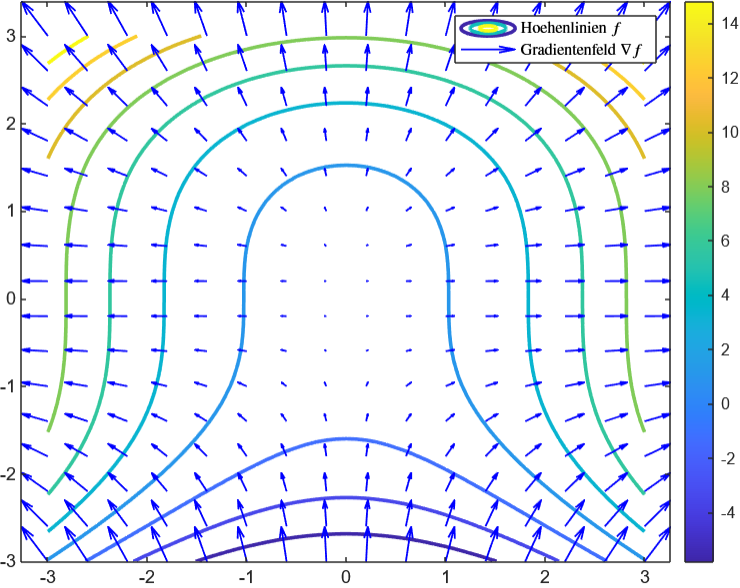
\includegraphics[width=0.6\textwidth]{../Multivariate_Analysis/Bilder/funktion_polynom_gradientenfeld.png}
	\caption{Visualisierung der H�henlinien und der Gradienten von \(f(x,y)=x^2+0.3\,y^3\) .}
\end{figure}

\begin{center}
\begin{tabular}{p{0.45\textwidth}|p{0.45\textwidth}}

\textbf{Matlab} &
\textbf{Python} \\

\begin{lstlisting}[language=Matlab]
x = -3:0.1:3;
y = -3:0.1:3;
[xx,yy] = meshgrid(x,y);
z = xx.^2 + 0.3*yy.^3;

contour(x,y,z,10,'LineWidth',2)
hold on

x = -3:0.4:3;
y = -3:0.4:3;
[xx,yy] = meshgrid(x,y);

g1 = 2*xx;
g2 = 9/10*yy.^2;

quiver(x,y,g1,g2,'b','LineWidth',1)

hold off
colorbar
legend({"Hoehenlinien $f$",
"Gradientenfeld $\nabla f$"},
"interpreter","latex")
\end{lstlisting}

&
\begin{lstlisting}[language=Python]
import numpy as np
import matplotlib.pyplot as plt

x = np.arange(-3,3.1,0.1)
y = np.arange(-3,3.1,0.1)
xx,yy = np.meshgrid(x,y)

z = xx**2 + 0.3*yy**3

plt.contour(x,y,z,10,linewidths=2)

x = np.arange(-3,3.1,0.4)
y = np.arange(-3,3.1,0.4)
xx,yy = np.meshgrid(x,y)

g1 = 2*xx
g2 = 0.9*yy**2

plt.quiver(x,y,g1,g2,color='b')

plt.colorbar()
plt.legend([r"H�henlinien $f$",
r"Gradientenfeld $\nabla f$"])

plt.show()
\end{lstlisting}

\end{tabular}
\end{center}

Streng genommen muss man sich fragen, inwiefern die partiellen Ableitungen separat garantieren, dass eine Funktion \(f\), die von $n$ Variablen abh�ngt, differenzierbar ist. Dies f�hrt zum Begriff der totalen Differenzierbarkeit. Wir k�nnen uns an dieser Stelle merken:  Wenn  in  einer  Umgebung eines \(\vec x^*\in D_f\)  alle  partiellen  Ableitungen von \(f\)  existieren und stetig sind, dann kann man die Funktion in \(\vec x^*\) in eine beliebige \textbf{Richtung} ableiten.

Eine beliebige Richtung wird per Definition durch einen \textbf{ Einheitsvektor } angegeben, also einen Vektor mit normierter Euklidischer L�nge.
    \[\hat v \in \mathbb R^n: \quad  \|\hat{ v}\|_2 = 1 \,.\]
    Wie nutzen im folgenden den kleinen Hut, um Einheitsvektoren zu kennzeichnen. Ist \(f\) in einer Umgebung von \(\vec x^*\in \mathbb R^n\) differenzierbar, so existiert der Grenzwert
    \begin{equation*} \lim\limits_{h\to 0} \dfrac{ f(\vec x^* - h\cdot \hat v)-f(\vec x^*)}{h}\end{equation*}
    und er hei�t Richtungsableitung von \(f\)  in \(\vec x^*\) in Richtung \(\hat v\) und bekommt das Symbol
    \[
    \dfrac{\partial f}{\partial \hat v}(\vec x^*) = \lim\limits_{h\to 0} \dfrac{ f(\vec x^* - h\cdot \hat v)-f(\vec x^*)}{h}\,.
    \]
    In der Praxis berechnet man den Grenzwert nicht, sondern macht sich zu Nutze, dass die Richtungsableitung von \(f\) in Richtung \(\hat v\) die Projektion des Gradienten \(\nabla f(\vec x^*)\) auf die Richtung \(\hat v\) ist:

    \begin{exabox}{Richtungsableitung von $f$}{ }
    \begin{equation}\label{MULTI-richtungsableitung}
    \dfrac{\partial f}{\partial \hat v}(\vec x^*) = \left\langle \nabla f(\vec x^*), \hat{\vec v}\right\rangle\,.
    \end{equation}
    \end{exabox}

    Die spitzen Klammern in \eqref{MULTI-richtungsableitung} bezeichnen das \textbf{Skalarprodukt} in \(\mathbb R^n\):
	  \[ \vec v, \vec u \in \mathbb R^n: \quad \left\langle \vec v,  \vec u \right\rangle  = \sum\limits_{i=1}^n v_i \cdot u_i \,.\]

 Es gilt also
    \[ \dfrac{\partial f}{\partial \hat v}(\vec x^*) = \left\langle \nabla f(\vec x^*), \hat v\right\rangle = \|\nabla f(\vec x^*)\|_2 \cdot \underbrace{ || \hat v||_2}_{\displaystyle{=1}} \cdot \cos(\alpha) \] und damit
    \[ \left\{ \begin{array}{rcl c rcl c rcl}
		    \alpha &=& 0  &\Rightarrow  & \cos(\alpha) &=& 1 & \Rightarrow & \hat v &=& \dfrac{\nabla f(\vec x^*)}{||\nabla f(\vec x^*)||_2}\,,\\[2ex]
		    \alpha &=& \pi & \Rightarrow & \cos(\alpha) &=& -1 & \Rightarrow & \hat v &=& -\dfrac{\nabla f(\vec x^*)}{||\nabla f(\vec x^*)||_2}\,.
    \end{array}\right.
    \]
    Die Eigenschaften des Gradienten sind also mathematisch fundiert - wir wiederholen sie:
    \begin{itemize}
	    \item Der Gradientenvektor zeigt immer in die Richtung des st�rksten Anstiegs von \(f\).
	    \item Der Gradientenvektor steht senkrecht auf den H�henlinien von \(f\).
		\item Der Gradientenvektor einer Funktion von $n$ Ver�nderlichen ist ein Vektor im $\mathbb R^n$. Er zeigt nicht aus der Ebene raus, sondern lebt, wie die H�henlinien, in der Ebene der Landkarte.
    \end{itemize}

    Das Konzept der Ableitung einer Funktion mehrerer Ver�nderlicher l��t sich �bertragen auf eine vektorwertige Funktion mehrerer Ver�nderlicher
    \[ \vec f: \mathbb R^n \to \mathbb R^n, \, \underbrace{\vec x}_{\left( \begin{array}{c} x_1 \\ \vdots \\ x_n \end{array}\right)}  \mapsto \underbrace{\vec f(\vec x)}_{\left( \begin{array}{c} f_1(\vec x) \\ f_2(\vec x)\\ \vdots \\ f_n(\vec x)\end{array}\right)}\,. \]
    Existieren f�r jede der Funktionen \(f_i: \mathbb R^n \to \mathbb R\) alle partiellen Ableitungen, so erh�lt man die Jacobi-Matrix von \(\vec f\), wenn man alle partiellen Ableitungen in einer Matrix zusammenfasst:
    \[ J = \left( \begin{array}{cccc}
			    \dfrac{\partial f_1}{\partial x_1} &  \dfrac{\partial f_1}{\partial x_2} & \cdots &  \dfrac{\partial f_1}{\partial x_n} \\[2ex]
			    \dfrac{\partial f_2}{\partial x_1} &  \dfrac{\partial f_2}{\partial x_2} & \cdots &  \dfrac{\partial f_2}{\partial x_n} \\
			    \vdots & \vdots &\vdots & \vdots \\
			    \dfrac{\partial f_n}{\partial x_1} &  \dfrac{\partial f_n}{\partial x_2} & \cdots &  \dfrac{\partial f_n}{\partial x_n}
	    \end{array}\right)\,.
    \]

    Die \(i\)-te Zeile der Jacobi-Matrix von \(\vec f\) ist gerade der Gradient der Funktion \(f_i\)!
    \[ J = \left( \begin{array}{cccc}
			    \textcolor{blue}{\dfrac{\partial f_1}{\partial x_1}} &  \textcolor{blue}{\dfrac{\partial f_1}{\partial x_2}} & \textcolor{blue}{\cdots} & \textcolor{blue}{\dfrac{\partial f_1}{\partial x_n}} \\[2ex]
			    \dfrac{\partial f_2}{\partial x_1} &  \dfrac{\partial f_2}{\partial x_2} & \cdots &  \dfrac{\partial f_2}{\partial x_n} \\
			    \vdots & \vdots &\vdots & \vdots \\
			    \dfrac{\partial f_n}{\partial x_1} &  \dfrac{\partial f_n}{\partial x_2} & \cdots &  \dfrac{\partial f_n}{\partial x_n}
	    \end{array}\right) = \left(\begin{array}{c} \textcolor{blue}{\left(\nabla f_1\right)^\intercal }\\[2ex]
	    \left(\nabla f_2\right)^\intercal \\ \vdots \\\left(\nabla f_n\right)^\intercal \end{array}\right)\,.
    \]

\section{Kettenregel}

Bis jetzt haben wir untersucht, wie sich eine Funktion \(f(\vec x)\) �ndert, wenn man eine einzelne Koordinate variiert oder sich in eine feste Richtung \(\hat v\) bewegt. In Anwendungen h�ngt der Punkt \(\vec x\) aber oft selbst wieder von einer anderen Gr��e ab, zum Beispiel von der Zeit, vom Radius oder von einem Winkel. Dann betrachtet man eine zusammengesetzte Funktion
\[
t \mapsto \vec x(t) \mapsto f(\vec x(t))\,.
\]
Die Frage lautet dann: Wie schnell �ndert sich der Funktionswert \(f(\vec x(t))\), wenn sich der Punkt \(\vec x(t)\) entlang einer Kurve durch den Definitionsbereich bewegt?

Genau das beantwortet die \textbf{Kettenregel f�r mehrere Variablen}. Sie sagt: Die �nderung des Funktionswerts entlang der Kurve ergibt sich aus dem Gradienten von \(f\) und der �nderungsrichtung der Kurve.

\begin{theorembox}{Kettenregel f�r \(f:\mathbb R^n \to \mathbb R\)}{}
Es sei
\[
f:\mathbb R^n \to \mathbb R
\]
differenzierbar und
\[
\vec x:\mathbb R \to \mathbb R^n,\qquad t \mapsto \vec x(t)
\]
differenzierbar. Dann ist auch die zusammengesetzte Funktion
\[
t \mapsto f(\vec x(t))
\]
differenzierbar und es gilt
\[
\frac{\mathrm d}{\mathrm dt}f(\vec x(t))
=
\left\langle \nabla f(\vec x(t)), \vec x\,'(t)\right\rangle .
\]
\end{theorembox}

\noindent
Die Kettenregel sagt also:
\begin{itemize}
\item \(\nabla f(\vec x(t))\) beschreibt die lokale �nderung der Funktion,
\item \(\vec x\,'(t)\) beschreibt die Bewegungsrichtung entlang der Kurve,
\item das Skalarprodukt beider Vektoren liefert die momentane �nderungsrate des Funktionswerts.
\end{itemize}

\begin{exabox}{Kettenregel entlang einer Kurve}{}
Betrachten wir die Funktion
\[
f(x,y)=x^2+y^2
\]
und die Kurve
\[
\vec x(t)=
\begin{pmatrix}
\cos(t)\\
\sin(t)
\end{pmatrix}.
\]
Dann gilt
\[
f(\vec x(t)) = \cos^2(t)+\sin^2(t)=1,
\]
also
\[
\frac{\mathrm d}{\mathrm dt}f(\vec x(t))=0.
\]

Dasselbe Ergebnis liefert die Kettenregel:
\[
\nabla f(x,y)=
\begin{pmatrix}
2x\\
2y
\end{pmatrix}
\]
also
\[
\nabla f(\vec x(t))=
\begin{pmatrix}
2\cos(t)\\
2\sin(t)
\end{pmatrix},
\qquad
\vec x\,'(t)=
\begin{pmatrix}
-\sin(t)\\
\cos(t)
\end{pmatrix}.
\]
Damit folgt
\[
\frac{\mathrm d}{\mathrm dt}f(\vec x(t))
=
\left\langle
\begin{pmatrix}
2\cos(t)\\
2\sin(t)
\end{pmatrix},
\begin{pmatrix}
-\sin(t)\\
\cos(t)
\end{pmatrix}
\right\rangle
=0.
\]

Das passt zur Geometrie:
Die Kurve l�uft auf einer H�henlinie von \(f\), also �ndert sich der Funktionswert nicht.
\end{exabox}

\noindent
Die Kettenregel wird sp�ter an mehreren Stellen wieder auftauchen:
bei Koordinatentransformationen, bei der Linearisierung vektorwertiger Funktionen und bei Bewegungen in Kraft- oder Potentialfeldern. F�r vektorwertige Funktionen f�hrt sie direkt zur Matrixschreibweise mit der Jacobi-Matrix.

\section{Lineare N�herung von Vektorfeldern}

Eine differenzierbare Funktion \(f\) l��t sich in jeder Stelle ihres Definitionsbereichs linearisieren und zwar durch ihre Tangentengerade \(t\):
\begin{theorembox}{Linearisierung \(f:\mathbb R \to \mathbb R\) (Ableitung)}{ }
	Es sei $f$ differenzierbar auf $D_f\subset \mathbb R$ und $x^*\in D_f$. Die Tangente \(t\) lautet
	    \[ t:D_f \to \mathbb R,\,  x \mapsto t(x) = f(x^*) + f'(x^*)(x-x^*)\,. \]
    \end{theorembox}

    Die lineare N�herung einer differenzierbaren Funktion $f$, die von zwei Ver�nderlichen abh�ngt, ist keine Gerade mehr, sondern eine Ebene, die sich an \(f\) tangential anschmiegt. Man nennt die Ebene Tangentialebene.
    Es sei $f$ differenzierbar auf $D_f\subset \mathbb R^2$ und $\vec x^*\in D_f$. Die Tangentialebene \(t\) lautet
	  \begin{eqnarray*}
		  t: D_f \to \mathbb R,\, \vec x\mapsto t(\vec x^*) = f(\vec x^*) + \textcolor{blue}{ \dfrac{\partial f}{\partial x_1}(x_1 - x^*_1) + \dfrac{\partial f}{\partial x_2}(x_2 - x^*_2)} \,,
  \end{eqnarray*}
	  wobei die blau eingef�rbten Terme das \textcolor{blue}{Skalarprodukt} (\emph{inner product}) zwischen dem Vektor \(\nabla f\) und dem Vektor \((\vec x-\vec x^*) \) ist:
		  \[ \left\langle \textcolor{blue}{\nabla f (\vec x^*), (\vec x- \vec x^*)}\right\rangle = \dfrac{\partial f}{\partial x_1}(\vec x^*)\cdot (x_1 - x^*_1) + \dfrac{\partial f}{\partial x_2}(\vec x^*)\cdot ( x_2 - x^*_2) \in \mathbb R\,.\]

  F�r eine Funktion, die von \(n\) unabh�ngigen Variablen abh�ngt, gilt entsprechend:

    \begin{theorembox}{Linearisierung \(f:\mathbb R^n \to \mathbb R\) (Gradient)}{ }
    Es sei $f$ differenzierbar auf $D_f\subset \mathbb R^n$ und $\vec x^*\in D_f$. Die Linearisierung \(t\) lautet
	  \begin{eqnarray*}
		  t: D_f \to \mathbb R,\, \vec x\mapsto t(\vec x^*) = f(\vec x^*) + \left\langle \nabla f (\vec x^*), (\vec x- \vec x^* )\right\rangle\,.
  \end{eqnarray*}
    \end{theorembox}

    Betrachten wir als n�chstes eine vektorwertige Funktion mit zwei Komponentenfunktionen, also
    \[ \vec f: \mathbb R^2 \to \mathbb R^2, \left( \begin{array}{c} x_1 \\ x_2 \end{array}\right) \mapsto \left( \begin{array}{c} f_1(x_1,x_2) \\ f_2(x_1,x_2)\end{array}\right)\,. \]
    \(\vec f\) l��t sich an jeder Stelle \( \vec x^* = (x^*_1, x^*_2)^\intercal \in D_f\) des Definitionsbereichs linearisieren und die Linearisierung lautet
	  \begin{eqnarray*}
		  \vec t: D_f \to \mathbb R^2,  \vec x \mapsto \vec t  \left( \vec x\right) = \vec f(\vec x^*) + \textcolor{blue}{ J(\vec x^*) \left(\vec x - \vec x^*\right)}\,,
	  \end{eqnarray*}
	  wobei \(J(\vec x^*)\) die Jacobi-Matrix von \(\vec f\) an der Stelle \(\vec x^*\) bezeichnet. Der blau eingef�rbte Term ist die folgende \textcolor{blue}{Matrix-Vektor-Multiplikation}:
	  \begin{eqnarray*}
		  \textcolor{blue}{ J(\vec x^*) \left(\vec x - \vec x^*\right)} &=&
    \left( \begin{array}{cc}
			    \dfrac{\partial f_1}{\partial x_1} &  \dfrac{\partial f_1}{\partial x_2}\\[2ex]
			    \dfrac{\partial f_2}{\partial x_1} &  \dfrac{\partial f_2}{\partial x_2}
	    \end{array}\right) \left( \begin{array}{c} x_1 - x^*_1 \\[2ex] x_2 - x^*_2\end{array}\right) \\&=&
	    \left( \begin{array}{c} \dfrac{\partial f_1}{\partial x_1} \cdot (x_1-x_1^*)  + \dfrac{\partial f_1}{\partial x_2} \cdot (x_2-x_2^*) \\[2ex]
    \dfrac{\partial f_2}{\partial x_1} \cdot (x_1-x_1^*)  + \dfrac{\partial f_2}{\partial x_2} \cdot (x_2-x_2^*) \end{array}\right) \in \mathbb R^2  \end{eqnarray*}

  \noindent \textbf{Bemerkungen:}
  \begin{itemize}
	  \item Die lineare N�herung eines Vektorfeldes \(\vec f\) ist selbst wieder ein Vektorfeld.
	  \item Die lineare N�herung von \(\vec f\) ist genau das Vektorfeld, dessen Eintr�ge die linearen N�herungen der Komponentenfunktionen sind.
  \end{itemize}

Und das Konzept l��t sich auch auf differenzierbare Vektorfelder beliebiger Dimension verallgemeinern.
\begin{theorembox}{Linearisierung \(\vec f:\mathbb R^n \to \mathbb R^n\) (Jacobi-Matrix)}{ }
	Es sei $\vec f$ differenzierbar auf $D_f\subset \mathbb R^n$ und $\vec x^*\in D_f$. Die Linearisierung \(\vec t\) lautet
	\begin{equation*}
		  \vec t: D_f \to \mathbb R^n, \;\vec x \mapsto \vec t(\vec x) = \vec f(\vec x^*)+  J\left(\vec x^*\right) \left( \vec x - \vec x^*\right) \,.
	  \end{equation*}
    \end{theorembox}


\newpage

\setcounter{def}{0} \setcounter{satz}{0} \setcounter{exa}{0}
\chapter{Lokale Analysis}\label{MULTI-lokale-analysis}

\begin{table}[H]
  \centering
  \begin{tabularx}{\textwidth}{@{}>{\raggedright\arraybackslash}X r@{}}
    \toprule
    \multicolumn{2}{c}{\textbf{�bersicht �ber Lernziele und Voraussetzungen}}\\
    \midrule
    \textbf{Lernziele} & \\[.5\normalbaselineskip]
    \tabitem den maximalen absoluten Fehler einer Funktion mehrerer Ver�nderlicher mit Hilfe des Gradienten absch�tzen & \\
    \tabitem Erwartungswert und Varianz einer Funktion approximativ bestimmen (Fehlerfortpflanzung) & \\
    \tabitem kritische Punkte einer Funktion durch Bestimmung des Gradienten berechnen & \\
    \tabitem lokale Extrema mit Hilfe der Hesse-Matrix klassifizieren & \\[.5\normalbaselineskip]
    \midrule
    \textbf{Voraussetzungen} & \\[.5\normalbaselineskip]
    \tabitem Erwartungswert und Varianz & \\
    \tabitem Determinanten &  \\
    \tabitem partielle Ableitungen und Gradienten & \abschnittsverweis{MULTI-funktionen-mehrerer-veraenderlicher}  \\
    \tabitem Tangentialebenen als lineare N�herung & \abschnittsverweis{MULTI-funktionen-mehrerer-veraenderlicher} \\
    \bottomrule
  \end{tabularx}
\end{table}

\section*{Leitidee}

Im vorherigen Kapitel haben wir Werkzeuge entwickelt, um Funktionen mehrerer
Ver�nderlicher lokal zu beschreiben: partielle Ableitungen, Gradient,
Jacobi-Matrix und Tangentialebene.

Diese Werkzeuge sind nicht nur mathematische Konstruktionen.
Sie erlauben es, konkrete Fragestellungen zu beantworten:

\begin{itemize}
\item Wie stark beeinflussen Messfehler den Funktionswert?
\item Wie breitet sich statistische Unsicherheit durch eine Rechnung aus?
\item An welchen Stellen besitzt eine Funktion Extremwerte?
\end{itemize}

Die zentrale Idee f�r die Beantwortung dieser Fragen ist:
Eine differenzierbare Funktion wird in einer Umgebung eines Punktes
durch ihre lineare N�herung (Taylorpolynom erster Ordnung) beschrieben.

Der Gradient liefert dabei die lokalen �nderungsraten,
aus denen sich Fehlerabsch�tzungen, Fehlerfortpflanzung
und Extremwertbedingungen ableiten lassen.

\section{Absoluter, gr��ter Fehler}

Angenommen, wir wissen, dass der Wert der Gr��e $x_1$ gleich $5.0$ mit einem absoluten gr��ten Fehler von $0.2$ ist, und dass der Wert der Gr��e $x_2$ gleich $3.0$ mit einem absoluten gr��ten Fehler von $0.3$ ist.

\begin{center}
	\textbf{In welchem Bereich liegt dann der Wert der Funktion $f(\vec x) := \dfrac{x_1}{1+x_2^2}$? }
\end{center}

Jetzt k�nnten wir �ber den Verlauf der Funktion nachdenken und zum Beispiel mit Monotonie argumentieren \ldots Eine andere Idee ist anstatt die Funktion zu analysieren ihre Tangentialebene zu untersuchen! Aber Vorsicht: Das ist nicht exakt! Man muss sich �berzeugen, dass die Tangentialebene dicht genug an der Funktion liegt. Die Gleichung der Tangentialebene an der Stelle $\vec x^* = (5,3)$ ist:
\begin{exabox}{Tangentialebene}{ }
	\begin{eqnarray*} \vec x^* = (5,3): \quad  t(\vec x) &=& f(\vec x^*) + \langle \nabla f(\vec x^*) , (\vec x - \vec x^*)\rangle \\
		&=& \dfrac{1}{2} + \frac{1}{10}\cdot (x_1-5) - \frac{3}{10} \cdot (x_2-3) \quad (*)\\
\end{eqnarray*}
\end{exabox}

Mit $x_1\in [4.8, 5.2]$ und $x_2\in [2.7,3.3]$ kann man aus $(*)$ den m�glichen Bildbereich der Tangentialebene ablesen:
\begin{exabox}{Gr��ter absoluter Fehler $f(\vec x)$}{ }
	\begin{eqnarray*}
		t(\vec x) \in \left[\frac12-\frac{1}{10}\cdot 0.2 - \frac{3}{10}\cdot 0.3, \; \frac12 + \frac{1}{10}\cdot 0.2 + \frac{3}{10}\cdot0.3\right]\,.
\end{eqnarray*}
\end{exabox}

Die folgende Fehlerabsch�tzung basiert auf einer grundlegenden Idee der Analysis.
Eine differenzierbare Funktion l�sst sich in einer Umgebung eines Punktes
durch ihr Taylorpolynom erster Ordnung approximieren:

\[
f(\vec x) \approx f(\vec x^*) +
\langle \nabla f(\vec x^*), \vec x-\vec x^* \rangle .
\]

Diese lineare N�herung entspricht geometrisch der Tangentialebene
an den Graphen der Funktion im Punkt \(\vec x^*\).
Betrachten wir

\[ f(\vec x)=x_1^2 + x_2^2  \]

Die Tangentialebene im Punkt  \( (1,1)\)  lautet
\[ t(\vec x) = 2 \cdot (x_1-1)+2\cdot (x_2-1)+2 \]
\begin{figure}[h]
\centering
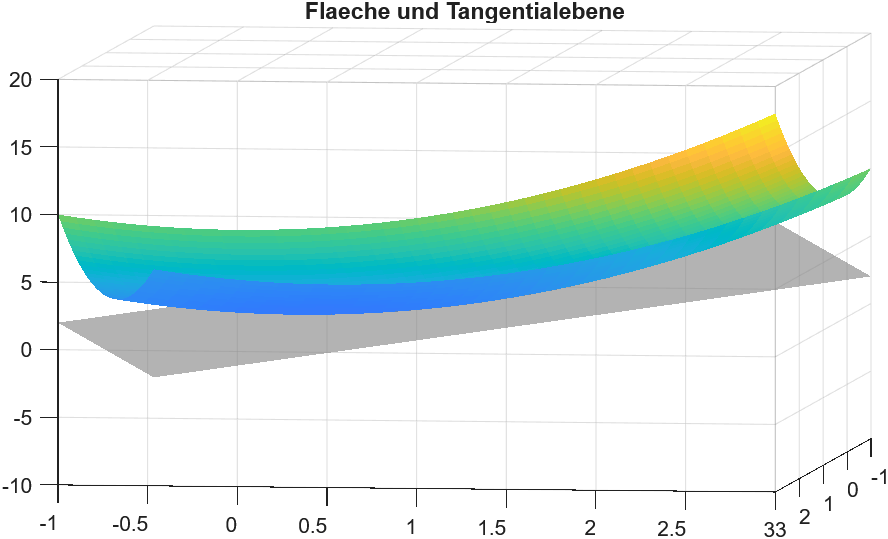
\includegraphics[width=0.6\textwidth]{../Multivariate_Analysis/Bilder/tangentialflaeche.png}
\caption{Linearisierung (Tangentialfl�che) schmiegt sich am Punkt \((1,1)\) an \(f\) an.}
\end{figure}

Mit Code kann man Fl�che und Tangentialebene vergleichen.

\begin{center}
\begin{tabular}{p{0.45\textwidth}|p{0.45\textwidth}}

\textbf{Matlab} &
\textbf{Python} \\

\begin{lstlisting}[language=Matlab]
x = -1:0.1:3;
y = -1:0.1:3;
[xx,yy] = meshgrid(x,y);

f = xx.^2 + yy.^2;
T = 2*(xx-1) + 2*(yy-1) + 2;

surf(xx,yy,f,'EdgeColor','none')
colormap parula
hold on

surf(xx,yy,T,...
'FaceColor',[0.5 0.5 0.5],...
'EdgeColor','none',...
'FaceAlpha',0.6)

hold off
title('Flaeche und Tangentialebene')
\end{lstlisting}

&
\begin{lstlisting}[language=Python]
import numpy as np
import matplotlib.pyplot as plt

x = np.arange(-1, 3.1, 0.1)
y = np.arange(-1, 3.1, 0.1)
xx, yy = np.meshgrid(x, y)

f = xx**2 + yy**2
T = 2*(xx-1) + 2*(yy-1) + 2

fig = plt.figure()
ax = fig.add_subplot( projection='3d')

ax.plot_surface(xx, yy, f, cmap='viridis')

ax.plot_surface(xx, yy, T, color='gray', alpha=0.6)

plt.title("Surface and tangent plane")
plt.show()
\end{lstlisting}

\end{tabular}
\end{center}

\vspace{0.5cm}

Die Formel zur Abschl�tzung des gr��ten m�glichen Fehlers in $f$ ergibt sich also aus der Taylorapproximation und sie lautet:
\begin{theorembox}{Gr��ter absoluter Fehler $f(\vec x)$}{ }
	\[ \Delta f = \left| \frac{\partial f}{\partial x_1} (\vec x^*) \right| \cdot \Delta x_1 + \left| \frac{\partial f}{\partial x_2} (\vec x^*) \right| \cdot \Delta x_2\,.\]
\end{theorembox}

\section{Standardabweichung}

In vielen Anwendungen sind die Eingangsgr��en einer Funktion nicht exakt bekannt,
sondern unterliegen zuf�lligen Schwankungen. Man modelliert sie daher als
\textbf{Zufallsgr��en}.

Wir betrachten zwei Zufallsgr��en
\[
X_1, X_2
\]
mit den Erwartungswerten
\[
E[X_1]=5, \qquad E[X_2]=3
\]
und den Standardabweichungen
\[
\sigma_{X_1}=0.1, \qquad \sigma_{X_2}=0.2 .
\]

Die Zufallsgr��en gehen in eine Funktion
\[
	f: \mathbb R^2 \to \mathbb R, (x_1,x_2) \mapsto \frac{x_1}{1+x_2^2}
\]
ein. Dadurch wird auch der Funktionswert selbst zu einer Zufallsgr��e

\[
f(X_1,X_2).
\]

Die Frage lautet nun:

\begin{center}
\textbf{Welchen Erwartungswert und welche Standardabweichung besitzt die Zufallsgr��e \(f(X_1,X_2)\)?}
\end{center}

Um diese Gr��en n�herungsweise zu bestimmen, ersetzen wir die Funktion
in der Umgebung des Erwartungswertes
\[
\vec x^*=(E[X_1],E[X_2])=(5,3)
\]
durch ihre Tangentialebene.
\begin{exabox}{Erwartungswert}{}
F�r kleine Schwankungen kann man die Funktion durch ihre lineare N�herung ersetzen:

\[
f(X_1,X_2)\approx
\frac12 + \frac{1}{10}(X_1-5)-\frac{3}{10}(X_2-3).
\]

Mit der Linearit�t des Erwartungswerts folgt

\[
E[f(X_1,X_2)]
=
\frac12
+\frac{1}{10}E[X_1-5]
-\frac{3}{10}E[X_2-3]
=\frac12 .
\]
\end{exabox}

Vorausgesetzt die Messgr��en $X_1$ und $X_2$ sind \textbf{unabh�ngig}, gilt f�r Varianz der Funktionswerte
\[\sigma^2_f=E[(f-E[f])^2]=E[f^2]-(E[f])^2\,. \]

\begin{exabox}{Varianz}{}

\[
\sigma_f^2
=
\frac{1}{100}\sigma_{X_1}^2
+
\frac{9}{100}\sigma_{X_2}^2 .
\]
\end{exabox}

Das Rezept ist also:
\begin{theorembox}{Fehlerfortpflanzung}{ }
	\begin{eqnarray*}
		\sigma_f^2 = \left( \frac{\partial f}{\partial x_1} (\vec x^*) \right)^2 \cdot \sigma_{x_1}^2  + \left( \frac{\partial f}{\partial x_2}(\vec x^*)\right)^2 \cdot \sigma_{x_2}^2\,.
	\end{eqnarray*}
\end{theorembox}

\section{Extrema von Funktionen zweier Ver�nderlicher}

Wie bei Funktionen von einer Ver�nderlichen untersucht man Stellen im Inneren des Definitionsbereichs, an denen der Funktionswert entweder gr��er oder kleiner ist als alle Funktionswerte in einer Umgebung: \textbf{lokale Maxima und Minima} (Sammelbegriff: Extrema). Der insgesamt gr��te oder kleinste Funktionswert hei�t das globale Maxiumum oder Minimum. Wenn es ein globales Maximum (Minimum) gibt (was nicht sein muss!), dann ist er entweder ein lokales Maxiumum (Minimum) oder ein Randwert, also ein Funktionswert, der auf dem Rand des Definitionsbereichs liegt. Man hat also eine hoffentlich �berschaubare Liste an Funktionswerten, aus der man den gr��ten bzw. den kleinsten suchen kann. Zum Finden von lokalen Extrema kann man Ableitungen benutzen.
H�nge \(f\) von zwei Variablen ab, haben kann man das sich geometrisch gut vorstellen: \textbf{ ein lokales Extremum liegt nur dort, wo die Tangentialebene horizontal ist}. Die Tangentialebene ist genau dann horizontal, wenn alle partiellen Ableitungen verschwinden! Das Verschwinden der partiellen Ableitungen ist also eine notwendige Bedingung f�r eine lokale Extremstelle:
\begin{theorembox}{Notwendige Bedingung f�r lokales Extremum}{ }
	\begin{eqnarray*}
		\frac{\partial f}{\partial x_1} (\vec x^*) = 0 \land \frac{\partial f}{\partial x_2} (\vec x^*) = 0  \; \Leftrightarrow  \; \nabla f(\vec x^*) = \vec 0 \,.
	\end{eqnarray*}
\end{theorembox}

Diese Bedingung ist zwar notwendig, beispielsweise verschwindet der Gradient der Funktion \(f: \mathbb R^2 \to \mathbb R, \vec x \mapsto x_1^2 + 0.3 \cdot x_2^3 \) an der Stelle \(\vec x^* = \vec 0\), aber trotzallem besitzt \(f\) dort kein lokales Extremum:
\begin{figure}[h]
\centering
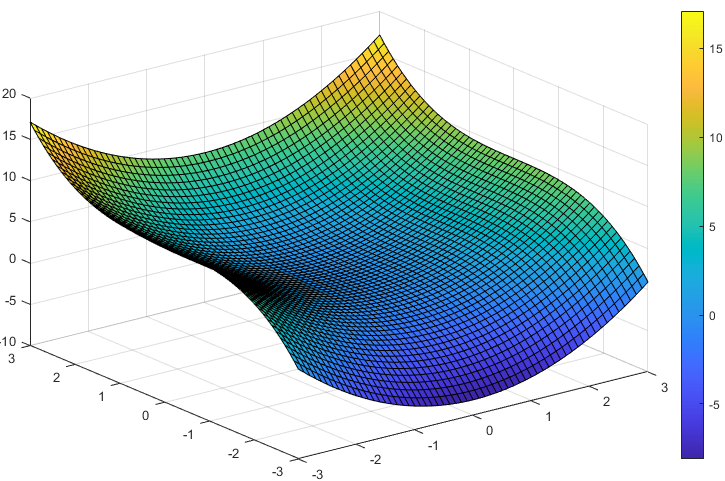
\includegraphics[width=0.6\textwidth]{../Multivariate_Analysis/Bilder/funktion_polynom_oberflaeche.png}
\caption{\(f\) besitzt am Usprung einen \textbf{Sattelpunkt}.}
\end{figure}

Meist, aber  nicht  immer,  kann  man  die  Lage  mit  der  zweiten  Ableitung aufkl�ren. Bei Funktionen einer Ver�nderlichen, kam es auf das Vorzeichen der zweiten Ableitung an. Mit zwei Ver�nderlichen kann man untersuchen, ob sich die Funktion in jede Richtung nach unten oder nach oben oder mal so und mal so von der Tangentialebene wegkr�mmt. Dazu bildet man die Matrix mit den Werten aller zweiten partiellen Ableitungen an der Stelle $\vec x^*$ - die sogenannte \textbf{Hesse-Matrix}:
	\begin{eqnarray*}
		H_f:= \left( \begin{array}{cc} \displaystyle{\frac{\partial^2 f}{\partial x_1^2}} (\vec x^*) & \displaystyle{\frac{\partial^2 f}{\partial x_1 \partial x_2}} (\vec x^*) \\
		\displaystyle{\frac{\partial^2 f}{\partial x_2 \partial x_1}} (\vec x^*) & \displaystyle{\frac{\partial^2 f}{\partial x_2^2}} (\vec x^*) \end{array}\right)
	\end{eqnarray*}

	Es gilt
	\begin{itemize}
		\item Ist \(f\) differenzierbar, dann ist die Hesse-Matrix symmetrisch.
		\item Sind alle Eigenwerte der Hesse-Matrix positiv, dann besitzt \(f\) ein lokales Minimum an der Stelle $\vec x^*$.
		\item Sind alle Eigenwerte der Hesse-Matrix negativ, dann besitzt \(f\) ein lokales Maximum an der Stelle $\vec x^*$.
		\item Sind die Eigenwerte null oder gemischt positiv und negativ, kann man ohne weitere Untersuchungen keine Aussage treffen.
	\end{itemize}

	Warum ist das so? �hnlich wie im eindimensionalen Fall, kann man ein Taylorpolynom vom Grad zwei anschauen\footnote{F�r eine Funktion einer Ver�nderlichen ist das die Schmiegeparabel \[f(x) = f(x_0) + f'(x_0)\cdot (x-x_0) + \frac12 \cdot f''(x_0)\cdot (x-x_0)^2 \]}

\begin{theorembox}{Taylorpolynom zweiten Grades}{ }
\[ z = f(\vec x^*) + \langle \nabla f (\vec x^*), (\vec x - \vec x^*)\rangle + \frac12 \cdot  \langle  H_f(\vec x^*) \, (\vec x - \vec x^*), \vec x - \vec x^*)\rangle  \,.  \]
\end{theorembox}

Der dritte Summand ist der quadratische Term und der sagt in erster N�herung aus, wie sich die Funktion \(f\) an die Tangentialebene (erster und zweiter Summand) schmiegt. F�r zwei Ver�nderliche ist es einfac die Vorzeichen der Eigenwerte ohne gro�e Rechnung zu pr�fen: Eine symmetrische $2\times 2$-Matrix hat genau dann Eigenwerte, die beide positiv oder aber beide negativ sind, wenn die Determinante der Matrix positiv ist:
\begin{theorembox}{Hinreichende Bedingung f�r lokales Extremum}{ }
	$H_f$ hat zwei Eigenwerte $\lambda_1, \lambda_2$ mit $\lambda_1 > 0 \land \lambda_2 > 0 \lor \lambda_1 < 0 \land \lambda_2 < 0: \Leftrightarrow
	 \mathrm{det} H_f = \lambda_1 \cdot \lambda_2 > 0 $
\end{theorembox}

Ist das der Fall, entscheidet das Vorzeichen des linken oberen Eintrags der Matrix, ob beide Eigenwerte positiv oder aber negativ sind.

Das Pr�fen auf ein lokales Extremum an $\vec x^* \in \mathbb R^2$ sieht also als Rezept so aus:
\begin{enumerate}
	\item Bestimme den Gradienten an der Stelle $\vec x^*$
		\begin{enumerate}
	\item Falls der Gradient nicht der Nullvektor ist, dann liegt kein lokales Extremum vor.
	\item Falls der Gradient der Nullvektor ist, dann bestimme die Hessematrix $H_f$ an der Stelle  $\vec x^*)$.
		\begin{enumerate}
			\item Falls die Determinante $\mathrm{det}\,H_f < 0$, dann liegt ein Sattelpunkt vor, also kein lokales Extremum,
			\item Falls die Determinante $\mathrm{det}\,H_f > 0$: es liegt ein Extremum vor.
			\item Falls die Determinante $\mathrm{det}\,H_f = 0$: keine Entscheidung m�glich, die Eigenwerte m�ssen berechnet werden.
		\end{enumerate}
	\end{enumerate}
\end{enumerate}

Die Funktion \[ f(x,y) = x^2 - y^2\] hat im Ursprung einen Sattelpunkt. Das H�henlinienprofil zeigt eine Hyperbelstruktur.

\begin{figure}[h]
\centering
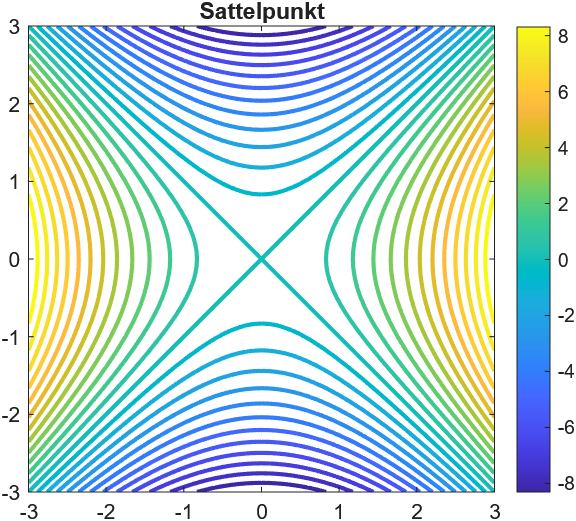
\includegraphics[width=0.6\textwidth]{../Multivariate_Analysis/Bilder/sattelpunkt.png}
\caption{\(f(x,y) =  x^2 - y^2\) besitzt am Usprung einen \textbf{Sattelpunkt}.}
\end{figure}

\begin{center}
\begin{tabular}{p{0.45\textwidth}|p{0.45\textwidth}}

\textbf{Matlab} &
\textbf{Python} \\

\begin{lstlisting}[language=Matlab]
x = -3:0.1:3;
y = -3:0.1:3;
[xx,yy] = meshgrid(x,y);

z = xx.^2 - yy.^2;

contour(x,y,z,25,'LineWidth',2)
colorbar
axis equal
title('Sattelpunkt')
\end{lstlisting}

&
\begin{lstlisting}[language=Python]
import numpy as np
import matplotlib.pyplot as plt

x = np.arange(-3, 3.1, 0.1)
y = np.arange(-3, 3.1, 0.1)
xx, yy = np.meshgrid(x, y)

z = xx**2 - yy**2

plt.contour(x, y, z, 25, linewidths=2)
plt.colorbar()
plt.gca().set_aspect('equal')
plt.title("Saddle point")
plt.show()
\end{lstlisting}

\end{tabular}
\end{center}

\vspace{0.5cm}
\section*{Takeaways}

\begin{itemize}
\item Eine differenzierbare Funktion l�sst sich lokal durch ihre
\textbf{lineare N�herung} beschreiben:
\[
f(\vec x) \approx f(\vec x^*) +
\langle \nabla f(\vec x^*), \vec x-\vec x^* \rangle .
\]

\item Der \textbf{Gradient} beschreibt, wie stark sich der Funktionswert
bei �nderungen der Eingangsgr��en ver�ndert.

\item \textbf{Lokale Extrema} k�nnen nur an Stellen auftreten,
an denen der Gradient verschwindet:
\[
\nabla f(\vec x^*)=\vec 0 .
\]

\item Mit Hilfe des Gradienten l�sst sich
\textbf{Fehlerabsch�tzungen} berechnen.

\item Mit Hilfe der Hesse-Matrix l�sst sich die
\textbf{Fehlerfortpflanzung} berechnen.

\end{itemize}

\newpage

\setcounter{def}{0} \setcounter{satz}{0} \setcounter{exa}{0}
\chapter{Koordinatensysteme}\label{MULTI-koordinatensysteme}

\begin{table}[H]
  \centering
  \begin{tabularx}{\textwidth}{@{}>{\raggedright\arraybackslash}X r@{}}
    \toprule
    \multicolumn{2}{c}{\textbf{�bersicht �ber Lernziele und Voraussetzungen}}\\
    \midrule
    \textbf{Lernziele} & \\[.5\normalbaselineskip]
    \tabitem geeignete Koordinatensysteme f�r typische Symmetrien ausw�hlen (kartesisch, polar, zylindrisch, kugelf�rmig) & \\
    \tabitem Punkte zwischen kartesischen und Polarkoordinaten umrechnen & \\
    \tabitem Punkte zwischen kartesischen und Zylinderkoordinaten umrechnen & \\
    \tabitem Punkte zwischen kartesischen und Kugelkoordinaten umrechnen & \\
    \tabitem Wertebereiche und Mehrdeutigkeiten der Winkelkoordinaten korrekt ber�cksichtigen & \\[.5\normalbaselineskip]
    \midrule
    \textbf{Voraussetzungen} & \\[.5\normalbaselineskip]
    \tabitem trigonometrische Funktionen &  \\
    \tabitem Polarkoordinaten in $\mathbb R^2$ bzw.\ $\mathbb C$ &  \\
    \bottomrule
  \end{tabularx}
\end{table}

\section*{Leitidee}

Viele Probleme zeigen eine Struktur von Zeilen und Spalten (Kristalle, Solarpanels, Manhattan, \ldots ). F�r diese sind die �blichen kartesischen (\emph{cartesian}) Koordinaten gut geeignet. Viele andere Probleme weisen aber andere Symmetrien auf, insbesondere kreisf�rmige (Rad, Planetenbahn, \ldots ), zylinderf�rmige (Flasche, Tank, \ldots ) oder kugelf�rmige (Erde, Ballon, Tank, \ldots ) und es stellt sich heraus, dass es daf�r geeignete Koordinatensysteme gibt.

\begin{exabox}{Manhatten vs Paris}{ }
	\centering
	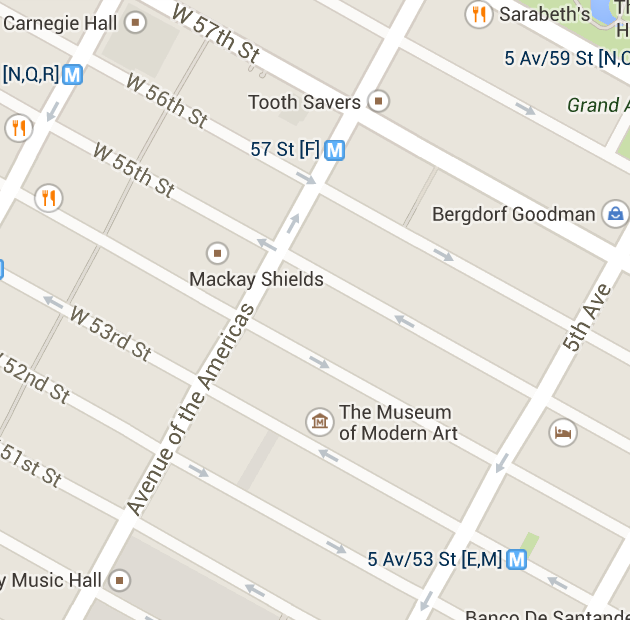
\includegraphics[width=0.3\textwidth]{../Multivariate_Analysis/Bilder/koordinaten_stadtplan_manhattan.png}\hspace{0.5cm}
	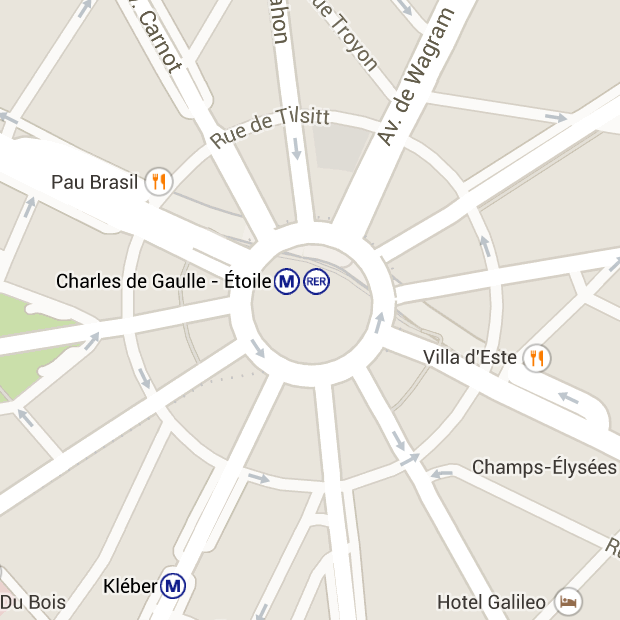
\includegraphics[width=0.3\textwidth]{../Multivariate_Analysis/Bilder/koordinaten_stadtplan_paris.png}
\end{exabox}

W�hlt man Koordinatensysteme, die der Problemstellung angepasst sind, dann k�nnen sich die Problemstellungen enorm vereinfachen! Es gibt drei Koordinatensysteme, die Sie immer wieder brauchen werden. Wir stellen sie jetzt vor.

\section{Polarkoordinaten}

Polarkoordinaten (\emph{polar coordinates}) kennen wir schon von den komplexen Zahlen: Statt einen Punkt im $\mathbb R^2$ als $(x,y)$ zu bestimmen, gibt man seinen Abstand $r$ vom Ursprung und den positiven oder negativen Winkel Azimut (\emph{azimuth}) $\varphi$ zur $x$-Achse an:

\begin{theorembox}{Polarkoordinaten $(r,\varphi)$}{ }
	\begin{minipage}{0.4\textwidth}
		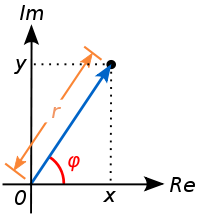
\includegraphics[width=0.7\textwidth]{../Multivariate_Analysis/Bilder/polarkoordinaten_komplexe_ebene.png}
\end{minipage}
\hspace{-2.3cm}\begin{minipage}{0.6\textwidth}
	\begin{itemize}
		\item Der Wertebereich der Koordinaten ist
	\begin{eqnarray*}
		r &\in& [0,\infty)\,,\\
		\varphi &\in& (-\pi,\pi]\,.
	\end{eqnarray*}
\item Umrechnung von Polar- auf kartesische Koordinaten $(r,\varphi) \Rightarrow (x,x)$:
	\begin{eqnarray*}
		x &=& r \cdot \cos(\varphi)\,,\\
		y &=& r \cdot \sin(\varphi)\,.
	\end{eqnarray*}
\item Umrechnung von kartesischen zu Polarkoordinaten $(x,y) \Rightarrow (r,\varphi)$:
	\begin{eqnarray*}
		r &=& \sqrt{x^2 + y^2}\,,\\
		\varphi &=& \mathrm{atan2}(y,x) + n\cdot 2\pi\,.
	\end{eqnarray*}
\end{itemize}
\end{minipage}
\end{theorembox}

\noindent Bemerkungen:\randverweis{MA1-komplexe-zahlen-grundlagen}
\begin{itemize}
	\item der Winkel $\varphi$ ist nur bis auf ein Vielfaches von $2\pi$ bestimmt!
	\item f�r $r=0$ ist der Winkel beliebig!
\end{itemize}

\section{Zylinderkoordinaten}

Man gibt zu den Polarkoordinaten in der $xy$-Ebene die �bliche $z$-Achse dazu und hat damit ein Koordinatensystem f�r den $\mathbb R^3$, die Zylinderkoordinaten (\emph{cylindrical coordinates}):
\begin{theorembox}{Zylinderkoordinaten $(r,\varphi, z)$}{ }
	\begin{minipage}{0.4\textwidth}
		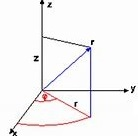
\includegraphics[width=0.7\textwidth]{../Multivariate_Analysis/Bilder/zylinderkoordinaten.png}
\end{minipage}
\hspace{-2.3cm}\begin{minipage}{0.6\textwidth}
	\begin{itemize}
		\item Der Wertebereich der Koordinaten ist
	\begin{eqnarray*}
		r &\in& [0,\infty)\,,\\
		\varphi &\in& (-\pi,\pi]\,,\\
		z &\in& \mathbb R\,.
	\end{eqnarray*}
\item Umrechnung von Zylinder- auf kartesische Koordinaten $(r,\varphi,z) \Rightarrow (x,x,z)$:
	\begin{eqnarray*}
		x &=& r \cdot \cos(\varphi)\,,\\
	y &=& r \cdot \sin(\varphi)\,,\\
	z &=& z\,.
\end{eqnarray*}
\item Umrechnung von kartesischen zu Zylinderkoordinaten $(x,y,z) \Rightarrow (r,\varphi,z)$:
\begin{eqnarray*}
	r &=& \sqrt{x^2 + y^2}\,,\\
	\tan(\varphi) &=& \frac{y}{x}\Rightarrow \varphi = \mathrm{atan2}(y,x) + n\cdot 2\pi\,, \\
		z &=& z\,.
	\end{eqnarray*}
\end{itemize}
\end{minipage}
\end{theorembox}

\section{Kugelkoordinaten}

Die Kugelkoordinaten (sph�rischen Koordinaten) (\emph{spherical coordinates}) sind eine andere Erweiterung der Polarkoordinaten ins Dreidimensionale. Statt der kartesischen $z$-Koordinate wie bei den Zylinderkoordinaten nimmt man hier den Polwinkel (Zenitwinkel) $\theta$ zur positiven $z$-Achse hinzu.
Anders als bei den Zylinderkoordinaten, misst der Radius $r$ den Abstand des betrachteten Punkts vom Ursprung und nicht nur die Projektion in die $xy$-Ebene:

\begin{theorembox}{Kugelkoordinaten $(r,\varphi, \theta)$}{ }
	\begin{minipage}{0.4\textwidth}
		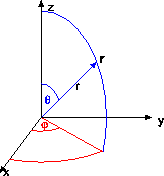
\includegraphics[width=0.7\textwidth]{../Multivariate_Analysis/Bilder/kugelkoordinaten.png}
\end{minipage}
\hspace{-2.3cm}\begin{minipage}{0.6\textwidth}
	\begin{itemize}
		\item Wertebereich f�r Radius, Azimut und Polwinkel
	\begin{eqnarray*}
		r &\in& [0,\infty)\,,\\
		\varphi &\in& (-\pi,\pi]\,,\\
		\theta &\in& [0, \pi]\,.
	\end{eqnarray*}
\item Umrechnung von  $(r,\varphi,\theta)$ auf $(x,x,z)$:
	\begin{eqnarray*}
		x &=& r \cdot \sin(\theta)\cdot \cos(\varphi)\,,\\
		y &=& r \cdot \sin(\theta)\cdot \sin(\varphi)\,,\\
		z &=& r\cdot \cos(\theta)\,.
	\end{eqnarray*}
\item Umrechnung von $(x,y,z)$ auf $(r,\varphi,z)$:
	\begin{eqnarray*}
		r &=& \sqrt{x^2 + y^2 + z^2}\,,\\
		\tan(\varphi) &=& \frac{y}{x} \Rightarrow \varphi = \mathrm{atan2}(y,x) + n\cdot 2\pi\,, \\
		\cos(\theta) &=& \frac{z}{r} \Rightarrow \theta = \arccos\left( \frac{z}{r}\right) \,,
	\end{eqnarray*}
\end{itemize}
\end{minipage}
\end{theorembox}


\newpage

\setcounter{def}{0} \setcounter{satz}{0} \setcounter{exa}{0}
\chapter{Integration in mehr Dimensionen}\label{MULTI-mehrdimensionale-integrale}

\begin{table}[H]
  \centering
  \begin{tabularx}{\textwidth}{@{}>{\raggedright\arraybackslash}X r@{}}
    \toprule
    \multicolumn{2}{c}{\textbf{�bersicht �ber Lernziele und Voraussetzungen}}\\
    \midrule
    \textbf{Lernziele} & \\[.5\normalbaselineskip]
    \tabitem Mehrfachintegrale geometrisch als Volumen oder Gesamtgr��e interpretieren & \\
    \tabitem kartesische Mehrfachintegrale durch iterierte Integration berechnen & \\
    \tabitem Integrationsbereiche geeignet parametrisieren & \\
    \tabitem Mehrfachintegrale in Polarkoordinaten, Zylinder- und Kugelkoordinaten berechnen & \\
    \tabitem Fl�chenintegrale als Integration einer Dichtegr��e �ber eine Fl�che interpretieren & \\[.5\normalbaselineskip]
    \midrule
    \textbf{Voraussetzungen} & \\[.5\normalbaselineskip]
    \tabitem bestimmte Integrale &  \\
    \tabitem Skalarprodukte & \\
    \tabitem partielle Ableitungen und Gradienten & \abschnittsverweis{MULTI-funktionen-mehrerer-veraenderlicher} \\
    \tabitem Koordinatentransformationen (polar, zylindrisch, sph�risch) & \abschnittsverweis{MULTI-koordinatensysteme}  \\
    \bottomrule
  \end{tabularx}
\end{table}

\section*{Leitidee}

Bisher haben wir Werkzeuge kennengelernt, mit denen sich das \emph{lokale Verhalten}
einer Funktion beschreiben l�sst: partielle Ableitungen, Gradient, Jacobi-Matrix
und Tangentialebene.

Viele Anwendungen interessieren sich jedoch nicht f�r lokale �nderungen,
sondern f�r \emph{Gesamtgr��en}. Beispiele sind:

\begin{itemize}
\item die Gesamtmasse eines K�rpers aus seiner Massendichte,
\item die gesamte elektrische Ladung aus einer Ladungsdichte,
\item die gesamte Energie aus einer Energiedichte,
\item das Volumen unter einer Fl�che.
\end{itemize}

Die zentrale Idee der Integralrechnung besteht darin,
eine solche Gesamtgr��e als Summe vieler kleiner lokaler Beitr�ge zu berechnen.

Bei Funktionen einer Ver�nderlichen summiert man Beitr�ge entlang einer Strecke.
Bei Funktionen mehrerer Ver�nderlicher summiert man Beitr�ge �ber Fl�chen oder
Volumen.

Mehrfachintegrale verallgemeinern also das eindimensionale Integral auf h�here
Dimensionen. Sie erlauben es, lokale Dichten �ber ihren gesamten Definitionsbereich
aufzusummieren und so globale Gr��en zu bestimmen.

Dabei spielen geeignete Koordinatensysteme eine wichtige Rolle.
W�hlt man Koordinaten, die zur Symmetrie eines Problems passen
(z.\,B. Polar-, Zylinder- oder Kugelkoordinaten),
werden viele Integrale deutlich einfacher.

\section{Berechnung kartesischer Mehrfachintegrale}

Das bestimmte Integral einer Funktion einer Ver�nderlichen gibt die Fl�che unter dem Funktionsgraphen an
\[ A = \int_a^b f(x) \, \mathrm d x\,.\]
\begin{figure}[h]
\centering
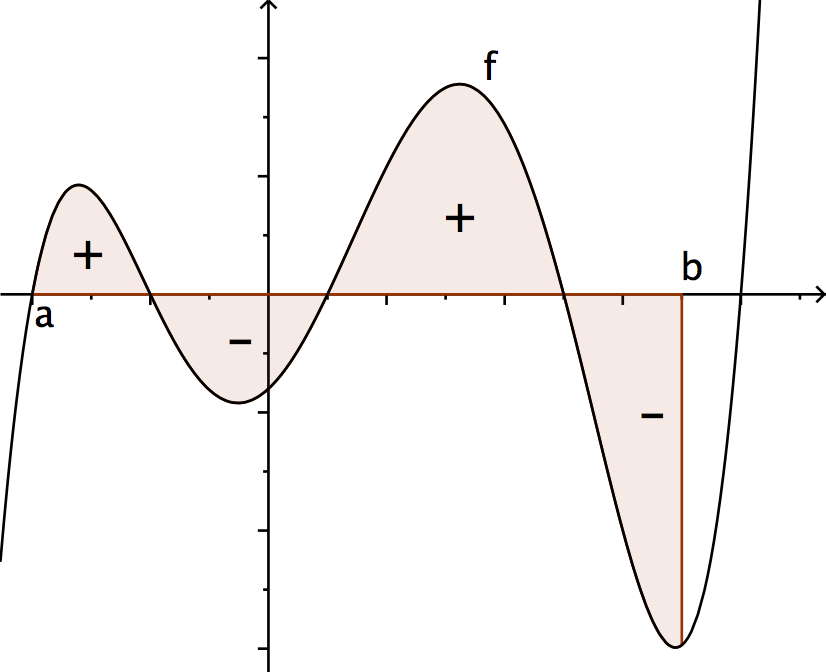
\includegraphics[width=0.4\textwidth]{../Multivariate_Analysis/Bilder/integral_flaecheninhalt.png}
\caption{Integral liefert den Fl�cheninhalt unter dem Graph von \(f(x)\).}
\end{figure}

\vspace{0.5cm}

Entsprechend gibt das Integral einer Funktion zweier Ver�nderlicher das Volumen unter dem Funktionsgraphen an. Der Integrationsbereich \(D\) ist nun eine Teilmenge des $\mathbb R^2$, das Differential eine infinitessimales Fl�chenst�ck \(\mathrm d A\). Um anzudeuten, dass man �ber eine Fl�che integriert schreibt man oft ein doppeltes Integralsymbol:
\[ V = \iint_D f(x,y) \, \mathrm d A\,.\]

\begin{figure}[h]
\centering
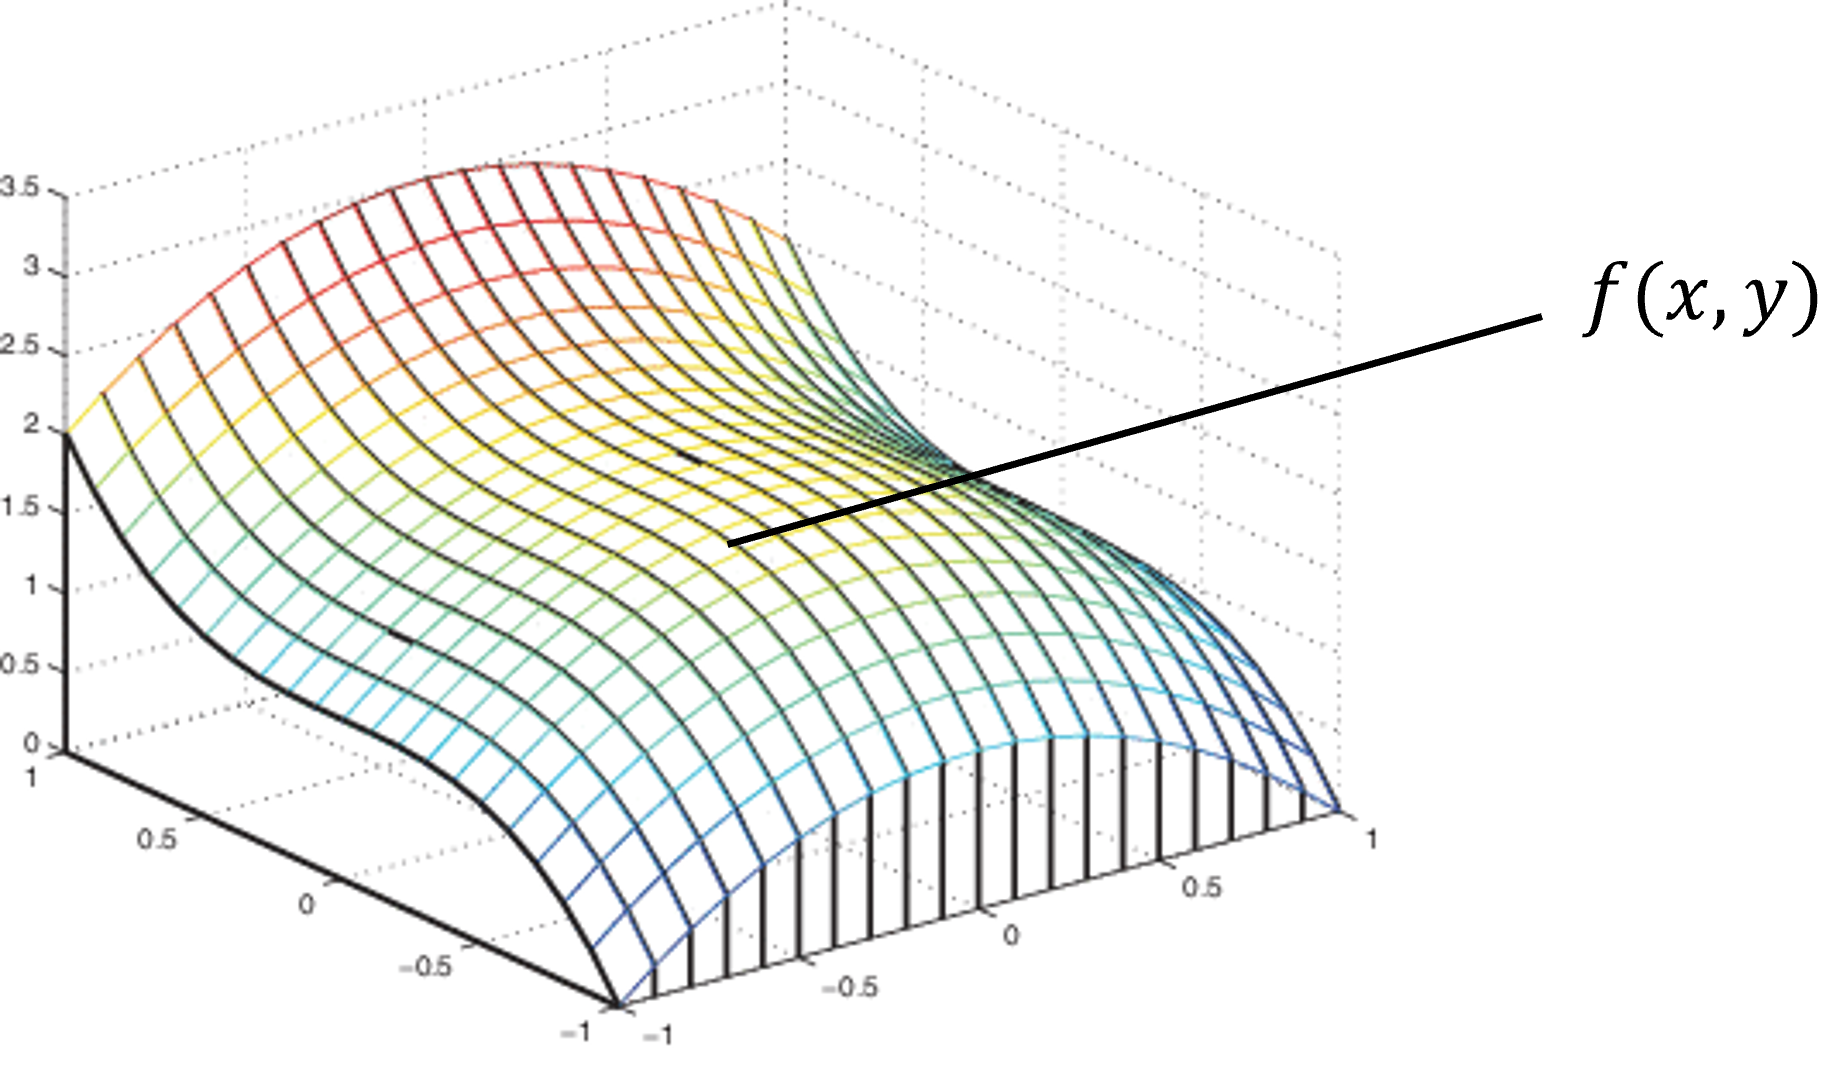
\includegraphics[width=0.5\textwidth]{../Multivariate_Analysis/Bilder/mehrfachintegral_volumen.png}
\caption{Integral liefert das Volumen unter dem Graph von \(f(x,y)\).}
\end{figure}

H�ngt eine Funktion von dreier  Ver�nderlichen ab, dann integrieren wir selbst �ber ein Volumen (darstellen kann man das dann leider nicht mehr gut). In der  Anwendung kommen Volumenintegrale aber  sehr h�ufig vor. M�chte man die Gesamtmasse eines Stoffes bestimmen, dessen Dichte von \(x,y\) und \(z\) abh�ngt, wobei der Stoff das Volumen \(V\) einnimmt, dann muss man �ber das Volumen \(V\) integrieren:
\[ M = \iiint_V \delta(x,y,z) \, \mathrm d V  \,.  \]

\begin{center}
\textbf{Wie integriert man �ber eine Fl�che oder ein Volumen?}
\end{center}

Angenommen, die Funktion $f(x,y):=x^2+y^2$ soll �ber das Dreieck zwischen den Punkten $(0|0)$, $(1|0)$ und $(0|1)$ integriert werden. Gesucht ist also sozusagen das Volumen eines dreieckigen Tortenst�cks unter dem Paraboloid:
\begin{figure}[h]
\centering
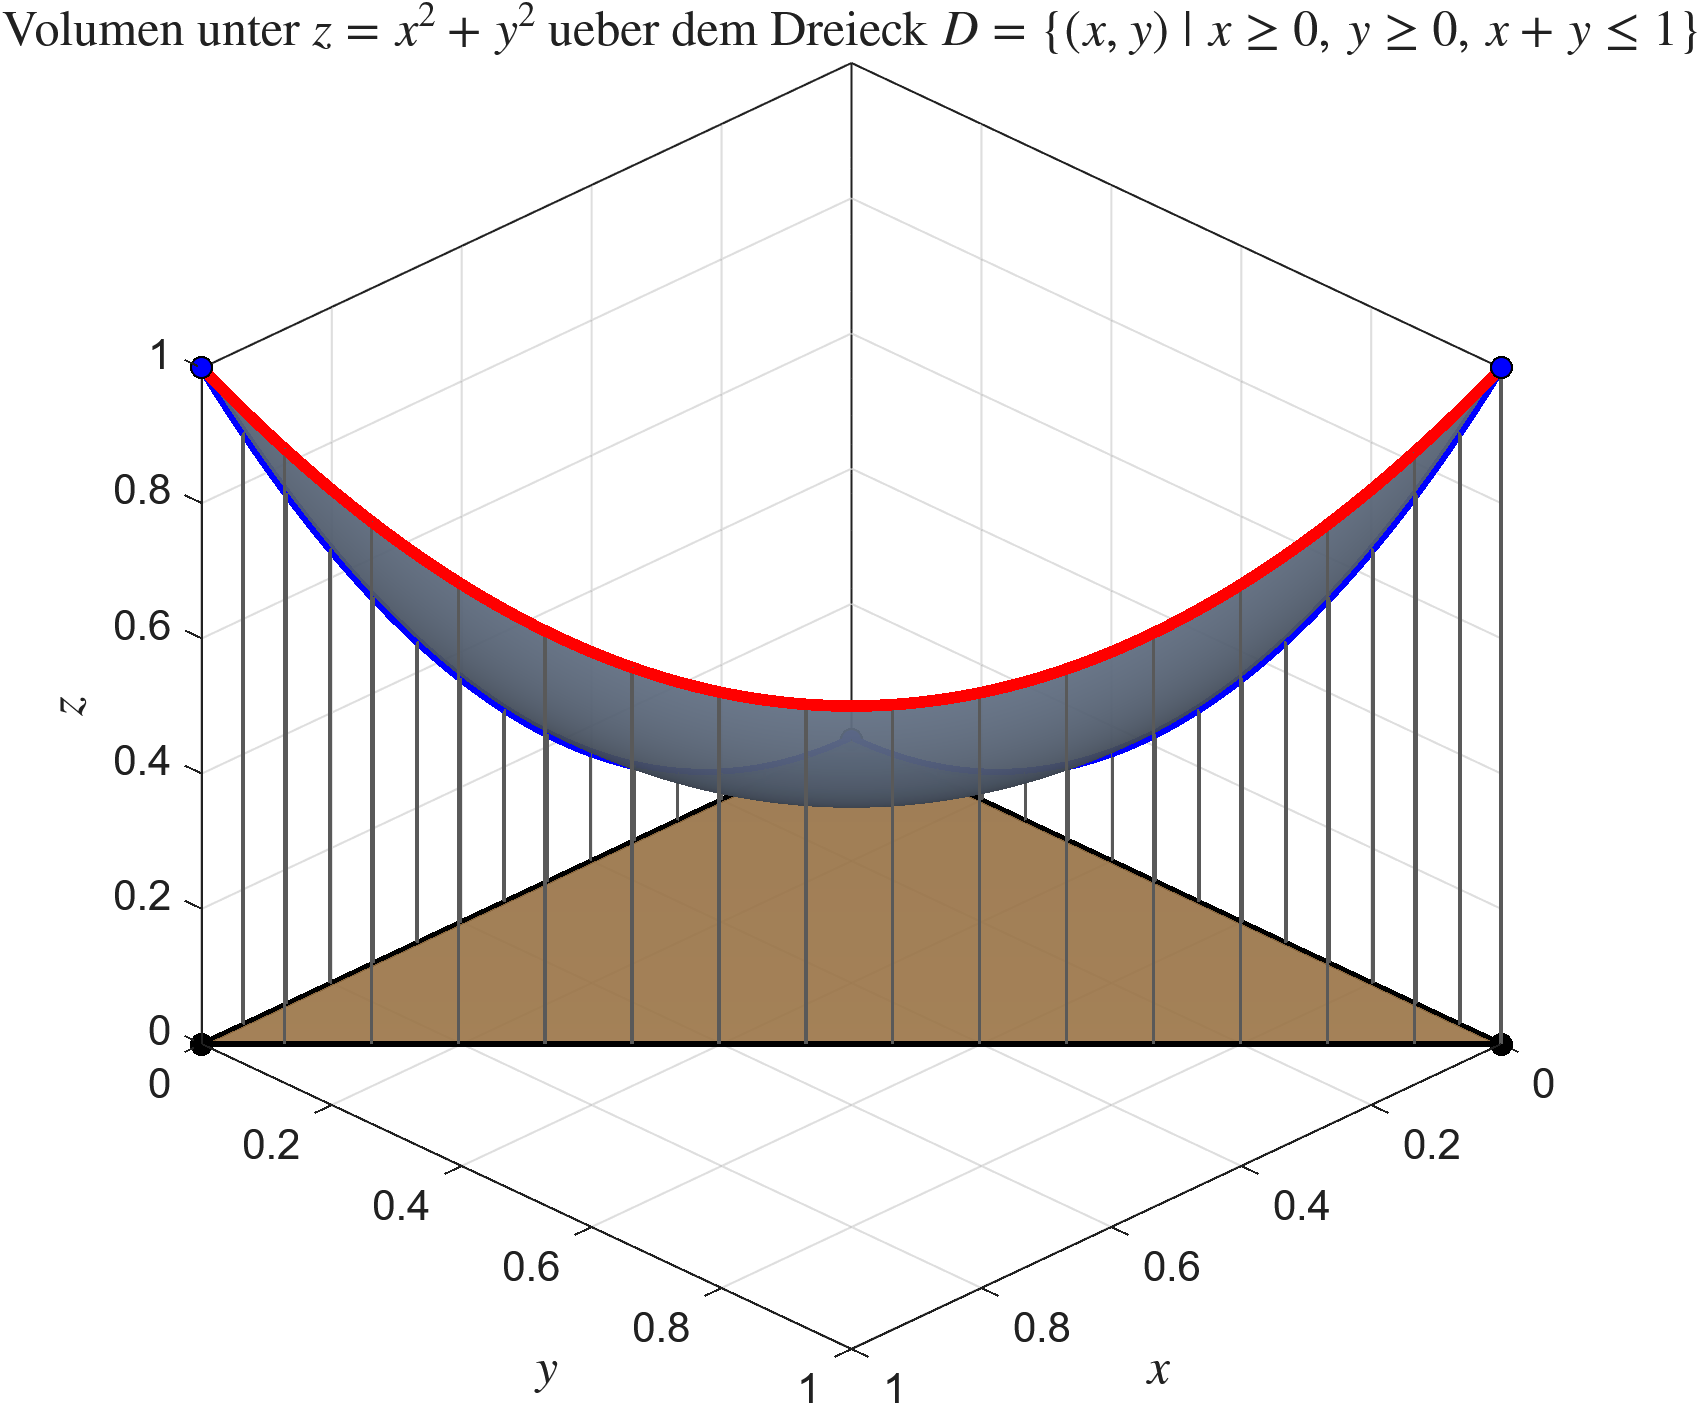
\includegraphics[width=0.5\textwidth]{../Multivariate_Analysis/Bilder/mehrfachintegral_dreieckiger_bereich.png}
\caption{Integral liefert das Volumen zwischen dreieckigem Integrationsgebiet und Paraboloid \(f(x,y)\).}
\end{figure}

Der �bliche Trick besteht nun darin, den Integrationsbereich
(d.\,h.\ das Dreieck) l�ngs der $x$- oder der $y$-Achse in
horizontale Salamischeiben zu schneiden, zum Beispiel so:
\[
D=\{(x,y)\mid 0\le x\le 1,\;0\le y\le 1-x\}.
\]

\begin{figure}[h]
\centering
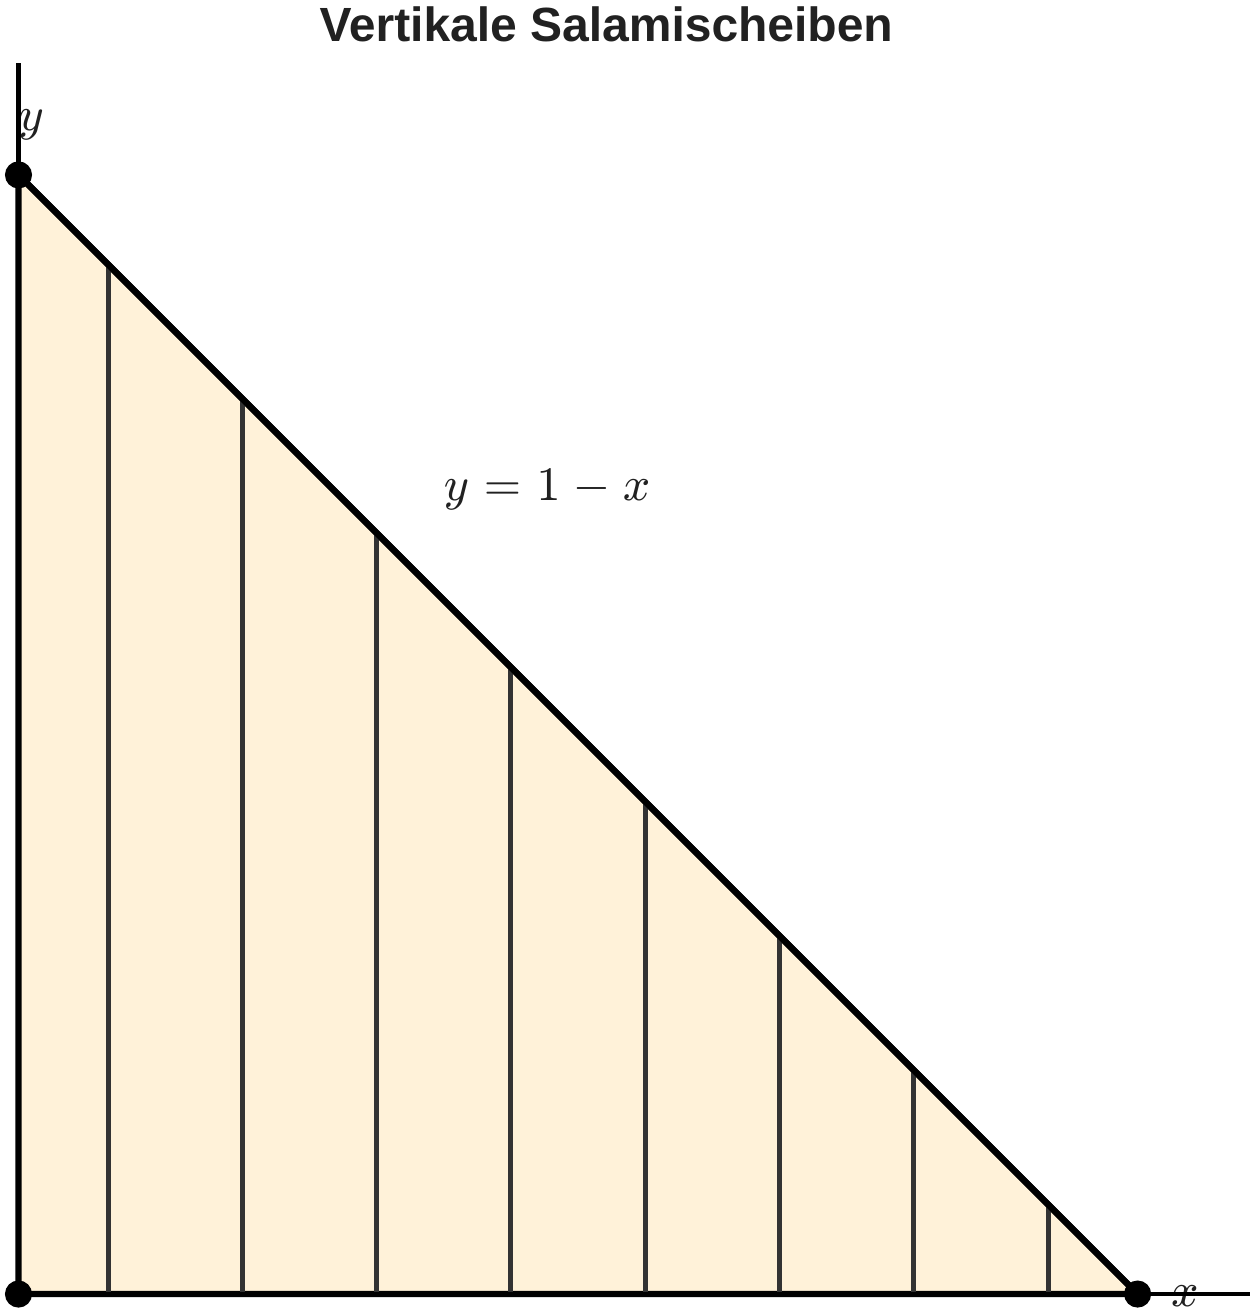
\includegraphics[width=0.4\textwidth]{../Multivariate_Analysis/Bilder/iterierte_integration_vertikale_schnitte.png}
\caption{Zerlegung des Integrationsgebiets in vertikale Scheiben: mache \(y\) von \(x\) abh�ngig.}
\end{figure}

Hierdurch kann man das Mehrfachintegral in ein eindimensionales
Integral eines eindimensionalen Integrals umwandeln, bei dem
die Grenzen des inneren Integrals von der Variablen des �u�eren
Integrals abh�ngen:
\[
\iint_D f(x,y)\,\mathrm dA
=
\int_0^1
\int_0^{1-x}
f(x,y)\,\mathrm dy\,\mathrm dx .
\]
Man k�nnte auch andersrum vorgehen und das Integrationsgebiet in horizontale Scheiben zerlegen: die Variable

\begin{figure}[h]
\centering
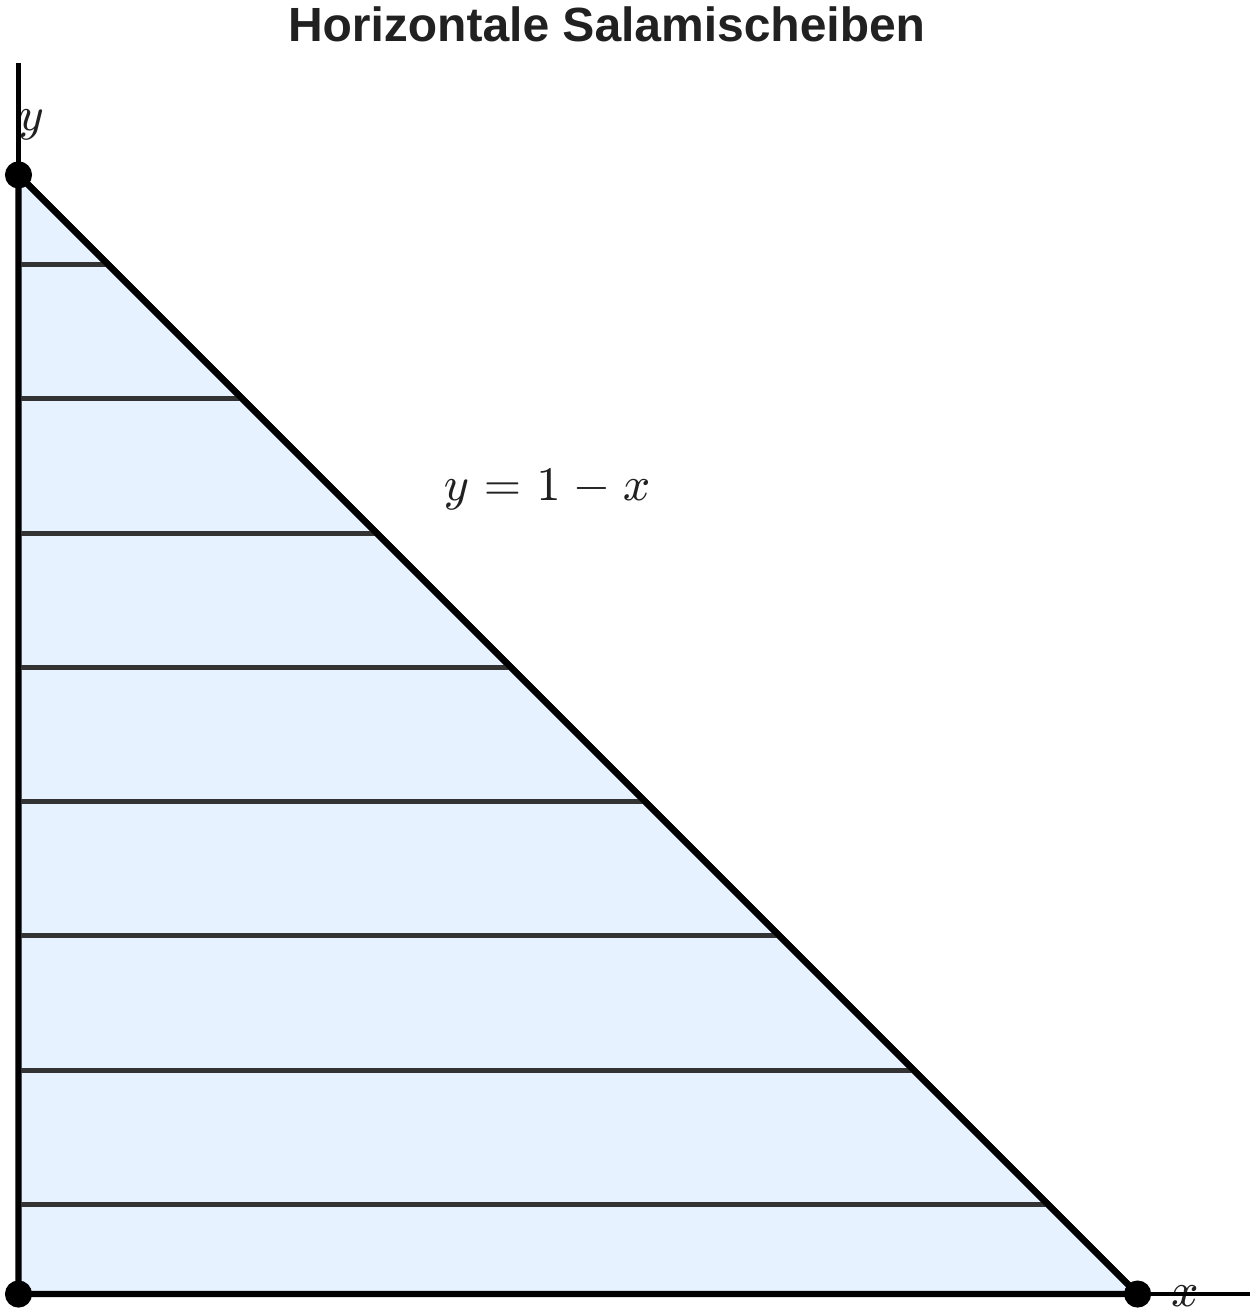
\includegraphics[width=0.4\textwidth]{../Multivariate_Analysis/Bilder/iterierte_integration_horizontale_schnitte.png}
\caption{Zerlegung des Integrationsgebiets in horizontale Scheiben: mache \(x\) von \(y\) abh�ngig.}
\end{figure}
Diese Zerlegung formuliert \(x\) in Abh�ngigkeit von \(y\):
\[
	D=\{(x,y)\mid 0\le y\le 1,\;0\le x\le 1-y\}\,,
\]
und entsprechend wird zuerst die Variable \(x\) aus und danach \(y\) ausintegriert:

\[
\iint_D f(x,y)\,\mathrm dA
=
\int_0^1 \int_0^{1-y} f(x,y)\,\mathrm dx\,\mathrm dy
\]

Auf dieselbe Weise werden Funktionen von drei und mehr
Ver�nderlichen integriert.

\section{ Integration in Polarkoordinaten und Zylinderkoordinaten}

Eine  Funktion $f(r,\varphi)$  und  ein  Integrationsbereich  seien  in  Polarkoordinaten gegeben. Dann m�chte man gerne �ber $r$ und $\varphi$ integrieren statt �ber $x$ und $y$. Wenn man sich die Integration als Grenzfall einer Summe vorstellt, summiert man in kartesischen Koordinaten hohe oder tiefe Quader mit kleiner quadratischer Grundfl�che $\mathrm{d}x \,\mathrm{d}y$ und H�he $\varphi(x,y)$. Bei Polarkoordinaten sind die Grundfl�chen dagegen nicht mehr quadratisch, sondern kleine Sektoren von Kreisringen. Die Fl�che eines solchen St�cks ist \textbf{nicht} $ \mathrm{d}r \,\mathrm{d}\varphi$, sondern verlangt einen Korrekturfaktor:
\[ \mathrm dx \, \mathrm dy = r \, \mathrm r \, \mathrm d \varphi\]

Damit ergibt sich f�r ein Fl�chenintegral in Polarkoordinaten

\[
\iint_A f(x,y)\,\mathrm dA
=
\iiint
f(r\,\cos(\varphi),
r\,\sin(\varphi)) \, r\,
\,\mathrm dr\,\mathrm d\varphi\,. \]

Die Fl�che einer Kreisscheibe mit Radius $R$ um den Ursprung wird zu einer fast trivialen Integrationsaufgabe:
\[A_{\textnormal{Kreis}} = \iint_S \,\mathrm d A = \int\limits_0^R \,\int\limits_0^{2\pi} r\,\mathrm d r \, \mathrm d \varphi = \dfrac12\, R^2 \cdot 2 \pi = \pi \, R^2\,. \]

In Zylinderkoordinaten ist derselbe Korrekturfaktor n�tig,
\[ \mathrm dx \, \mathrm dy \, \mathrm d z = r \, \mathrm r \, \mathrm d \varphi \, \mathrm d z\]

Damit ergibt sich f�r ein Volumenintegral in Zylinderkoordinaten

\[
	\iiint_V f(x,y,z)\,\mathrm dV
=
\iiint
f(r\,\cos(\varphi),
r\,\sin(\varphi), z) \, r\,
\,\mathrm dr\,\mathrm d\varphi \, \mathrm d z\,. \]

\section{Integration in Kugelkoordinaten}

Die Integration einer Funktion �ber ein Volumen $V$ kann man sich als Grenzwert
von Summen �ber kleine Teilvolumina vorstellen. Zerlegt man den Raum in kleine
Quader der Gr��e $\Delta x \,\Delta y\,\Delta z$, erh�lt man die Riemannsumme

\[
\int_V f(x,y,z)\,\mathrm dV
=
\lim_{n\to\infty}
\sum_{k=1}^n
f(x_k,y_k,z_k)\,\Delta x\,\Delta y\,\Delta z .
\]

Die Faktoren $\Delta x\,\Delta y\,\Delta z$ sind dabei die Volumina der kleinen
kartesischen W�rfel.

Verwendet man statt kartesischer Koordinaten Kugelkoordinaten
\[
(r,\theta,\varphi),
\]
so wird der Raum nicht mehr durch W�rfel, sondern durch kleine gekr�mmte
Volumenelemente zerlegt. F�r hinreichend kleine Schritte
$\mathrm dr$, $\mathrm d\theta$, $\mathrm d\varphi$
kann man dieses Volumen n�herungsweise aus den lokalen
Kantenl�ngen bestimmen.

In radialer Richtung hat das Volumenelement die L�nge $\mathrm dr$.
In Richtung des Polarwinkels $\theta$ entspricht eine Winkel�nderung
$\mathrm d\theta$ der Bogenl�nge $r\,\mathrm d\theta$.
In Richtung des Azimutwinkels $\varphi$ entsteht die Bogenl�nge
$r\sin\theta\,\mathrm d\varphi$.

Multipliziert man diese drei lokalen Kantenl�ngen, erh�lt man das
Volumenelement

\[
\mathrm dV
=
\mathrm dr \, (r\,\mathrm d\theta) \, (r\,\sin(\theta)\,\mathrm d\varphi)
=
r^2\, \sin (\theta)\,\mathrm dr\,\mathrm d(\theta)\,\mathrm d(\varphi)\, .
\]

Damit ergibt sich f�r ein Volumenintegral in Kugelkoordinaten

\[
\iiint_V f(x,y,z)\,\mathrm dV
=
\iiint
f(r\,\sin(\theta) \,\cos(\varphi),
  r\,\sin(\theta) \,\sin(\varphi),
  r\,\cos(\theta) )
\, r^2\sin\theta
\,\mathrm dr\,\mathrm d\theta\,\mathrm d\varphi\,. \]

Das Volumen einer Kugel l�sst sich sehr einfach bestimmen, denn \(f=1\):
\[
\iiint_V \,\mathrm dV
=
\iiint\mathrm dr\,\mathrm d\theta\,\mathrm d\varphi = \dfrac13\, R^3 \cdot (-\cos(\pi) + \cos(0)) \cdot 2 \pi = \dfrac43 \,\pi \, R^3\,. \]

\subsection*{Anwendungen}

In der Elektrotechnik beschreibt die Stromdichte
\[
\vec J(\vec r)
\]
die elektrische Stromst�rke pro Fl�cheneinheit.
Ihre Einheit ist
\[
\mathrm{A/m^2}.
\]

Die Stromdichte ist also eine \emph{Fl�chendichte} des Stroms:
Sie gibt an, wie viel Strom durch eine infinitesimal kleine
Fl�che flie�t.

Betrachtet man ein kleines Fl�chenelement $\mathrm dA$
mit Normalenvektor $\vec n$, so ist der durch dieses
Element flie�ende Strom

\[
\mathrm dI
=
\vec J \cdot \vec n \,\mathrm dA.
\]

Der gesamte Strom durch eine Querschnittsfl�che $A$
ergibt sich durch Aufsummieren aller lokalen Beitr�ge:

\[
I
=
\int_A \vec J \cdot \vec n \,\mathrm dA.
\]

Das Fl�chenintegral wandelt also eine lokale Dichtegr��e
(Strom pro Fl�che) in die globale Gesamtgr��e Strom um.

\bigskip

\textbf{Strukturelle Analogie:}

\[
\text{Strom} = \int \text{Stromdichte} \,\mathrm d(\text{Fl�che})
\]

Vergleich:

\[
\text{Energie} = \int \text{Leistung} \,\mathrm dt
\]

\[
\text{Masse} = \int \text{Massendichte} \,\mathrm dx
\]

In allen F�llen wird eine lokale Intensit�ts- oder Dichtegr��e
�ber ihren Bezugsraum integriert, um die zugeh�rige Gesamtgr��e
zu erhalten.

\newpage

\setcounter{def}{0} \setcounter{satz}{0} \setcounter{exa}{0}
\section*{Leitidee: Von lokalen �nderungen zu globalen Gr��en}\label{MULTI-leitidee}

Viele pyhsikalische, technische und wirtschaftliche Systeme h�ngen nicht nur von einer, sondern von mehreren Einflussgr��en ab - beispielsweise

\begin{itemize}
	\item Die Leistung eines Motors h�ngt von Drehzahl und Drehmoment ab.
	\item Die Dichte eines Materials kann von Ort und Temperatur abh�ngen.
	\item Die Energie eines Systems h�ngt von mehreren Zusatandvariablen ab.
\end{itemize}

Mathematisch beschreibt man solche Zusammenh�nge durch Funktionen mehrerer Ver�nderlicher

\[ f: \mathbb R^n \to \mathbb R, \vec x \mapsto f\left( \vec x\right)\,.\]

Die zentrale Idee der Analysis bleibt dabei dieselbe wie bei Funktionen einer Ver�nderlichen:

\begin{center}
	\textbf{Lokale �nderungen bestimmen das Verhalten des gesamten Systems.}
\end{center}

Die wichtigsten Werkzeuge daf�r sind

\begin{itemize}
	\item partielle Ableitungen,
	\item der Gradient,
	\item die lineare N�herung (Tangentialebene),
	\item Mehrfachintegrale.
\end{itemize}

Dieses Skript f�hrt in diese Grundideen der \textbf{multivariaten Analysis} ein.

\newpage

\end{document}
